%!TEX root = main.tex
\documentclass[a4paper,12pt]{article}

% The packages are useful for many mathematical symbols but you may well not need them
\usepackage{amsmath,amssymb,amscd}

\usepackage{caption}
% \usepackage{subcaption}
\usepackage[justification=RaggedRight,
            format=hang]{subcaption}
\usepackage{hyperref}
\let\subsectionautorefname\sectionautorefname
\let\subsubsectionautorefname\sectionautorefname

% This is great for reading in images
\usepackage{graphicx}
\usepackage{footnote}
\captionsetup[subfigure]{width=0.9\textwidth}

\usepackage[backend=bibtex,style=authoryear,maxcitenames=2, natbib=true]{biblatex} % Use the bibtex backend with the authoryear citation style (which resembles APA)
\usepackage{array}
\usepackage[makeroom]{cancel}
\usepackage{algorithm}
\usepackage[noend]{algpseudocode}

\addbibresource{library.bib}

% This is great for drafts as it will show all the labels you have defined.
% DON'T forget to comment it out before submission
%\usepackage{showkeys}

% Change Page Size
\typeout{--- Increasing width and height of text }
% A4 paper is 297mm high and 210mm wide.
\setlength{\textwidth}{16.00cm} % OK for both Letter and A4
\setlength{\oddsidemargin}{-0.04cm}  % actual margins = 1inch + \oddsidemargin
                                 %top/odd/even-sidemargin
\setlength{\evensidemargin}{-0.04cm} %  ditto
\setlength{\topmargin}{-1.0cm}      %  ditto
\setlength{\headheight}{18pt} \setlength{\headsep}{6pt}
\setlength{\topskip}{0pt}  %see pp155 also about baselineskip
\setlength{\textheight}{23.0cm} % 25cm for A4, 23cm for Letter or DJ
\setlength{\footskip}{0.7cm}

\begin{document}

\title{Networks Project: Numerical analysis of the Barab\'asi-Albert Model}
\date{26th March, 2017}
\author{Lingyi Hu\\ CID: \texttt{00919977}}
\maketitle

\vspace*{2cm}
\noindent
{\bf Abstract:} In this report, we investigate the degree distribution of the Barab\'asi-Albert (BA) Model and 2 other related variants, namely the random attachment and preferential attachment through random walks. We derive the degree distribution and the theoretical largest expected degree, $k_1$, for preferential and random attachment and compare it against numerical simulation. Agreement of the numerical results with the theoretical model is investigated using the Kolmogorov-Smirnov test. The degree distribution of the random walk model is compared with the scaled free behaviour of the BA model and also with the geometric degree distribution of the random attachment model. 


\vspace*{2cm}
\noindent
{\bf Word count:}
2598 words in report (excluding front page, figure captions, table captions, acknowledgement and bibliography).


\newpage

%!TEX root = ../main.tex
\section{Introduction}\label{section:introduction}

The Barab\'asi-Albert (BA) model is a model for generating scale-free networks with a preferential attachment mechanism \citep{Barabasi1999}. It has been extensively studied in many fields, albeit under different names, for its resemblance to real-world networks such as the internet and citation networks, and is the basic model underlying the concept of ``the rich get richer", or more accurately, ``the rich get richer quicker". The fat tail is a central characteristic in the model, which implies that there are a few vertices with very high degree, while most vertices have below average degree. In this model, every new vertex that joins attaches itself to existing vertices with a probability proportional to its degree, so that vertices with a higher degree are more likely to further increase its degree count, leading to a scale free degree distribution. 

There are two key parts to this model: growth and preferential attachment. The random attachment model is a limiting case of the BA model where it retains growth but does not include preferential attachment. Here we show that the resulting degree distribution in this limit is no longer scale-free but geometric, suggesting that growth alone is not enough to produce a power law distribution. 

Recent works \citep{Saramaki2004,Cannings2013,J.P.Saramaki2004} have also investigated if preferential attachment can be reproduced without a global knowledge of the entire network, by performing a random walk on th graph, since such knowledge is impractical for real-world systems. In this project we briefly look at the of such a model and whether it reproduces the power law for preferential attachment. 
%!TEX root = ../main.tex
\section{Pure preferential attachment}\label{section:pure-preferential-attachment}

\subsection{Degree distribution: Theory}\label{subsection:ppa-degree-distribution}
The master equation that describes the evolution of the BA model is given by

\begin{equation}
	n(k, t+1) = n(k, t) + m \Pi(k-1, t)n(k-1, t) - m \Pi(k, t)n(k, t) + \delta_{k,m}
	\label{eq:master}
\end{equation}
where $k$ is the total degree of a vertex, $n(k, t)$ is the number of nodes at time $t$ with total degree $k$, and the probability $\Pi$ for choosing the existing vertex depends on the model. 

In the pure preferential attachment model, we choose an existing edge with $\Pi_{pa} \propto k$, which after normalizing gives $\Pi_{pa} = k/ 2E(t)$ where $E(t)$ is the number of edges and $2E(t)$ is the normalization constant corresponding to the total degree of the network. Assuming $E(0) = mN(0)$, the number of edges at a given time $t$ is given by $E(t) = mN(t)$, so we get $\Pi = k / 2mnN(t)$. Since we are concerned with the degree distribution of the model at large $t$, we consider the long-time ansatz $n(k, t) \rightarrow N(t) p_{\infty}(k)$. 

Substituting these terms into the master equation, we obtain 
\begin{equation}
	p_{\infty}(k) = \frac{1}{2}[(k-1)p_{\infty}(k-1) - kp_{infty}(k)] + \delta_{k,m}
	\label{eq:degree-distribution-p-infinity}
\end{equation}

It is clear that $p_{\infty}(k < m) = 0$, since $m$ edges are added at every stage. So there are 2 cases to consider when solving for the above equation: $k = m$ and $k > m$. 

We first consider the case when $k > m$. In this case, $\delta_{k,m} = 0$ and we can rearrange \autoref{eq:degree-distribution-p-infinity} to get

\begin{equation}
	\frac{p_{\infty}(k)}{p_{\infty}(k+1)} = \frac{k-1}{k+2}
	\label{eq:p-infinity-k-greater-m}	
\end{equation}

To solve this equation, we can substitute in a trial solution of the form

\begin{equation}
	f(z) = A \frac{\Gamma(z+1+a)}{\Gamma(z+1+b)}
	\label{eq:trial-solution}
\end{equation}
where $\Gamma(z)$ is the Gamma function, which is an extension of the factorial function, with its argument shifted by one, to all real and complex nnumbers except the non-positive integers. Its central property is that
\begin{equation}
	\Gamma(z+1) = z \Gamma(z),\,\, \Gamma(1) = 1.
	\label{eq:gamma-function-property}
\end{equation}

Substituting the trial solution in \autoref{eq:trial-solution} gives
\begin{equation}
	\frac{A \Gamma(z+1+a)}{\Gamma(z+1+b)} \times \frac{\Gamma(z+b)}{A \Gamma(z+a)}
\end{equation}
which indeed simplifies to give $(z+a) / (z+b)$, using the the property in \autoref{eq:gamma-function-property} that $\Gamma(z+a+1) / \Gamma(z+a) = z+a$. 

Substituting $a = -1$ and $b=2$, we get the solution for \autoref{eq:p-infinity-k-greater-m} in terms of $A$ and the Gamma function:

\begin{equation}
	p_{\infty}(k) = A \frac{\Gamma(k)}{\Gamma(k+3)}
\end{equation}
which simplifies to 
\begin{equation}
	p_{\infty}(k) = \frac{A}{k(k+1)(k+2)}.
	\label{eq:p-infinity-solution-unknown-A}
\end{equation}

For the second case of $k = m$, \autoref{eq:degree-distribution-p-infinity} becomes 
\begin{equation}
	p_{\infty}(m) = \frac{1}{2}[(m+1)p_{\infty}(m-1) - mp_{\infty}(m)] + 1. 
	\label{eq:p-infinity-k-equals-m}
\end{equation}
However, we already know that $p_{\infty}(k < m) = 0$, that is, $p_{\infty}(m-1) = 0$. Using this, and rearranging \autoref{eq:p-infinity-k-equals-m}, we get 

\begin{equation}
	p_{\infty}(m) = \frac{2}{m+2}.
	\label{p-infinity-normalization}
\end{equation}

Substituting $k = m$ and \autoref{p-infinity-normalization} into \autoref{eq:p-infinity-solution-unknown-A}, we get 

\begin{equation}
	\frac{A}{m(m+1)(m+2)} = \frac{2}{m+2}, 
\end{equation}
giving us the constant $A$ as
\begin{equation}
	A = 2m(m+1).
	\label{eq:normalization-constant}
\end{equation}

For this constant to be physically reasonable, we need to check that the probability satisfies normalization, that is, we need to prove
\begin{equation}
	\sum_{k=m}^\infty p_{\infty}(k) = 2m(m+1)\sum_{k=m}^\infty \frac{1}{k(k+1)(k+2)} = 1. 
	\label{eq:normalization-criteria}
\end{equation}

The term in the summation of \autoref{eq:normalization-criteria} can be expanded as a partial fraction:
\begin{equation}
	\sum_{k=m}^\infty \frac{1}{k(k+1)(k+2)} = \sum_{k=m}^\infty \frac{1}{2k} - \sum_{k=m}^\infty \frac{1}{k+1} + \sum_{k=m}^\infty \frac{1}{2(k+2)}
	\label{eq:partial-fractions}
\end{equation}

By writing out the first few terms of each summation, we can see that most terms cancel:

\begin{equation}
\setlength{\arraycolsep}{0pt}% no padding
\newcolumntype{B}{>{{}}c<{{}}}
\begin{array}{ B l B l B l B l B l B}
	\frac{1}{2m} & {}-{} &\frac{1}{m+1} & {}+{} & \cancel{\frac{1}{2(m+2)}} & \\
	& {}+{} & \frac{1}{2(m+1)} & {}-{} &\cancel{\frac{1}{m+2}} & {}+{} &\cancel{\frac{1}{m+3}} \\
	& & & {}+{} & \cancel{\frac{1}{2(m+2)}} & {}-{} & \cancel{\frac{1}{m+3}} & {}+{} &\frac{1}{2(m+4)} \\
	& & & & & {}+{}& \cancel{\frac{1}{2(m+3)}} & {}-{} & \frac{1}{m+4} & {}+{} & \frac{1}{2(m+5)} \\
	& & & & & & & {}+{}& ...\\
\end{array}
\label{eq:summation-cancel}
\end{equation}
and from the remaining terms we get the relation in \autoref{eq:normalization-criteria}
\begin{equation}
	 \sum_{k=m}^\infty p_{\infty}(k) = 2m(m+1)\left ( \frac{1}{2m} - \frac{1}{m} + \frac{1}{2(m+1)} \right ) = 2m(m+1) \frac{1}{2m(m+1)} = 1
	 \label{eq:normalization-satisfied}
\end{equation}

Hence, we can confirm that the complete exact solution for the probability distribution in the long time limit is 
\begin{equation}
	p_{\infty}(k) = \frac{2m(m+1)}{k(k+1)(k+2)}.
	\label{eq:p-infinity-solution}
\end{equation}

\subsection{Degree distribution: Numerical analysis}\label{subsection:ppa-numerical-analysis}

To leverage its speed, \texttt{c++} code was used to generate graph data, while \texttt{python} was used for data analysis due to its wide range of data analysis tools, such as \texttt{numpy}, \texttt{scipy}, and \texttt{pandas}. 

There were two main concerns when doing the numerical simulation:

\begin{enumerate}
	\item What should the initial graph $G_0$ be? 
	\item Should self loops and multiple edges be allowed?
	\item Of what order should $m$ and $N$ be respectively?
\end{enumerate}

The initial graph should be negligible if $N \rightarrow \infty$. In our simulations, we assumed that the $N$ chosen was large enough for this limit to apply, so we for convenience we chose our initial graph to be an empty graph. 

Computational efficiency of our algorithm is important considering that bigger datasets give better and more reliable statistical results. To yield statistically significant results and optimize efficiency, the following algorithm was used. In this algorithm, the array $M$ holds the list of edges represented by pairs of vertices, for example, the vertices at $M[0]$ and $M[1]$ are connected, $M[2]$ and $M[3]$ are connected, and so on. In this list, the number of occurences of a vertex is equal to its degree, so it can be used as a sample pool to achieve preferential attachment. To choose $m$ neighbours for each new vertex, we then sample from $M$. This is also equivalent to choosing an edge at random and then choosing a vertex at random from the edge. 

\begin{algorithm}
\caption{Algorithm for preferential attachment}\label{alg:pa}
\begin{algorithmic}[1]
\Require{number of vertices $N$, minimum degree $m$}\Comment{$N > m$}
\State Initialize our graph $g$
\State Initialize $M$ as an empty array of length $2Nm$
\For{$v$ in [0, ..., n-1]}
	\State add new vertex to $g$
	\For{$i$ in [0, ..., m-1]}
		\State $M[2(vm + i)] \gets v$
		\State draw $r$ uniformly at random 
		\State from $[0, ..., 2(vm + i)]$\Comment{Choose random vertex from $M$}
		\State $M[2(vm + i)+1] \gets M[r]$ \Comment{Add edge between vertex $M[r]$ and $v$}
	\EndFor
\EndFor
\State
\For{$i$ in [0, ..., nm-1]}\Comment{Add all edges stored in M into the graph}
	\State Add edge $(M[2i], M[2i+1])$ to graph $g$
\EndFor
\end{algorithmic}
\end{algorithm}

Clearly this approach produces self loops and multiple edges. However, since we are concerned with the limit of $N \rightarrow \infty$, these effects are insignificant. Also, while unsatisfactory, multiple edges and self-loops do not affect our theoretical result. In the large $N$ limit, the probability of getting multiple edges or self loops is small, and so for simplicity this algorithm was used without modification. 

$N$ was mostly limited by efficiency and storage space to be $10^7$, and $m$ was chosen to vary between $1$ and $32$. 

To check that the model was implemented correctly, the degree distribution generated by the model compared checked against the \texttt{networkx} implementation of the BA model. By using the same random seed, we could check that degree distribution between the two models were exactly the same. Graphs of fewer than $10$ nodes were also generated and visualized to ensure that the points followed some basic constraints. This gives confidence that the algorithm is working as expected. 

To investigate the degree distribution, the model was run for fixed $N$ but varying $m$. Several numerical runs were performed for each set of values to improve statistics. It was found that generally above $N=10^4$, finite size scaling effects are insignificant (see \autoref{subsection:pa-numerical-largest-degree}). In order to reduce finite size effects, $N=10^6$ was used. 

As $N$ is finite, there is bound to be a noisy tail at large $k$, where these degrees appeared once. To reduce the noise, 100 simulations were run for a single $m$ and the degree distribution was averaged over all runs. This can be seen in \autoref{fig:pa-fixed-n-degree-dist}. The log-binning technique \citep{Christensen:2005} was adopted to to collapse the noisy data. 

\begin{figure}
    \centering
    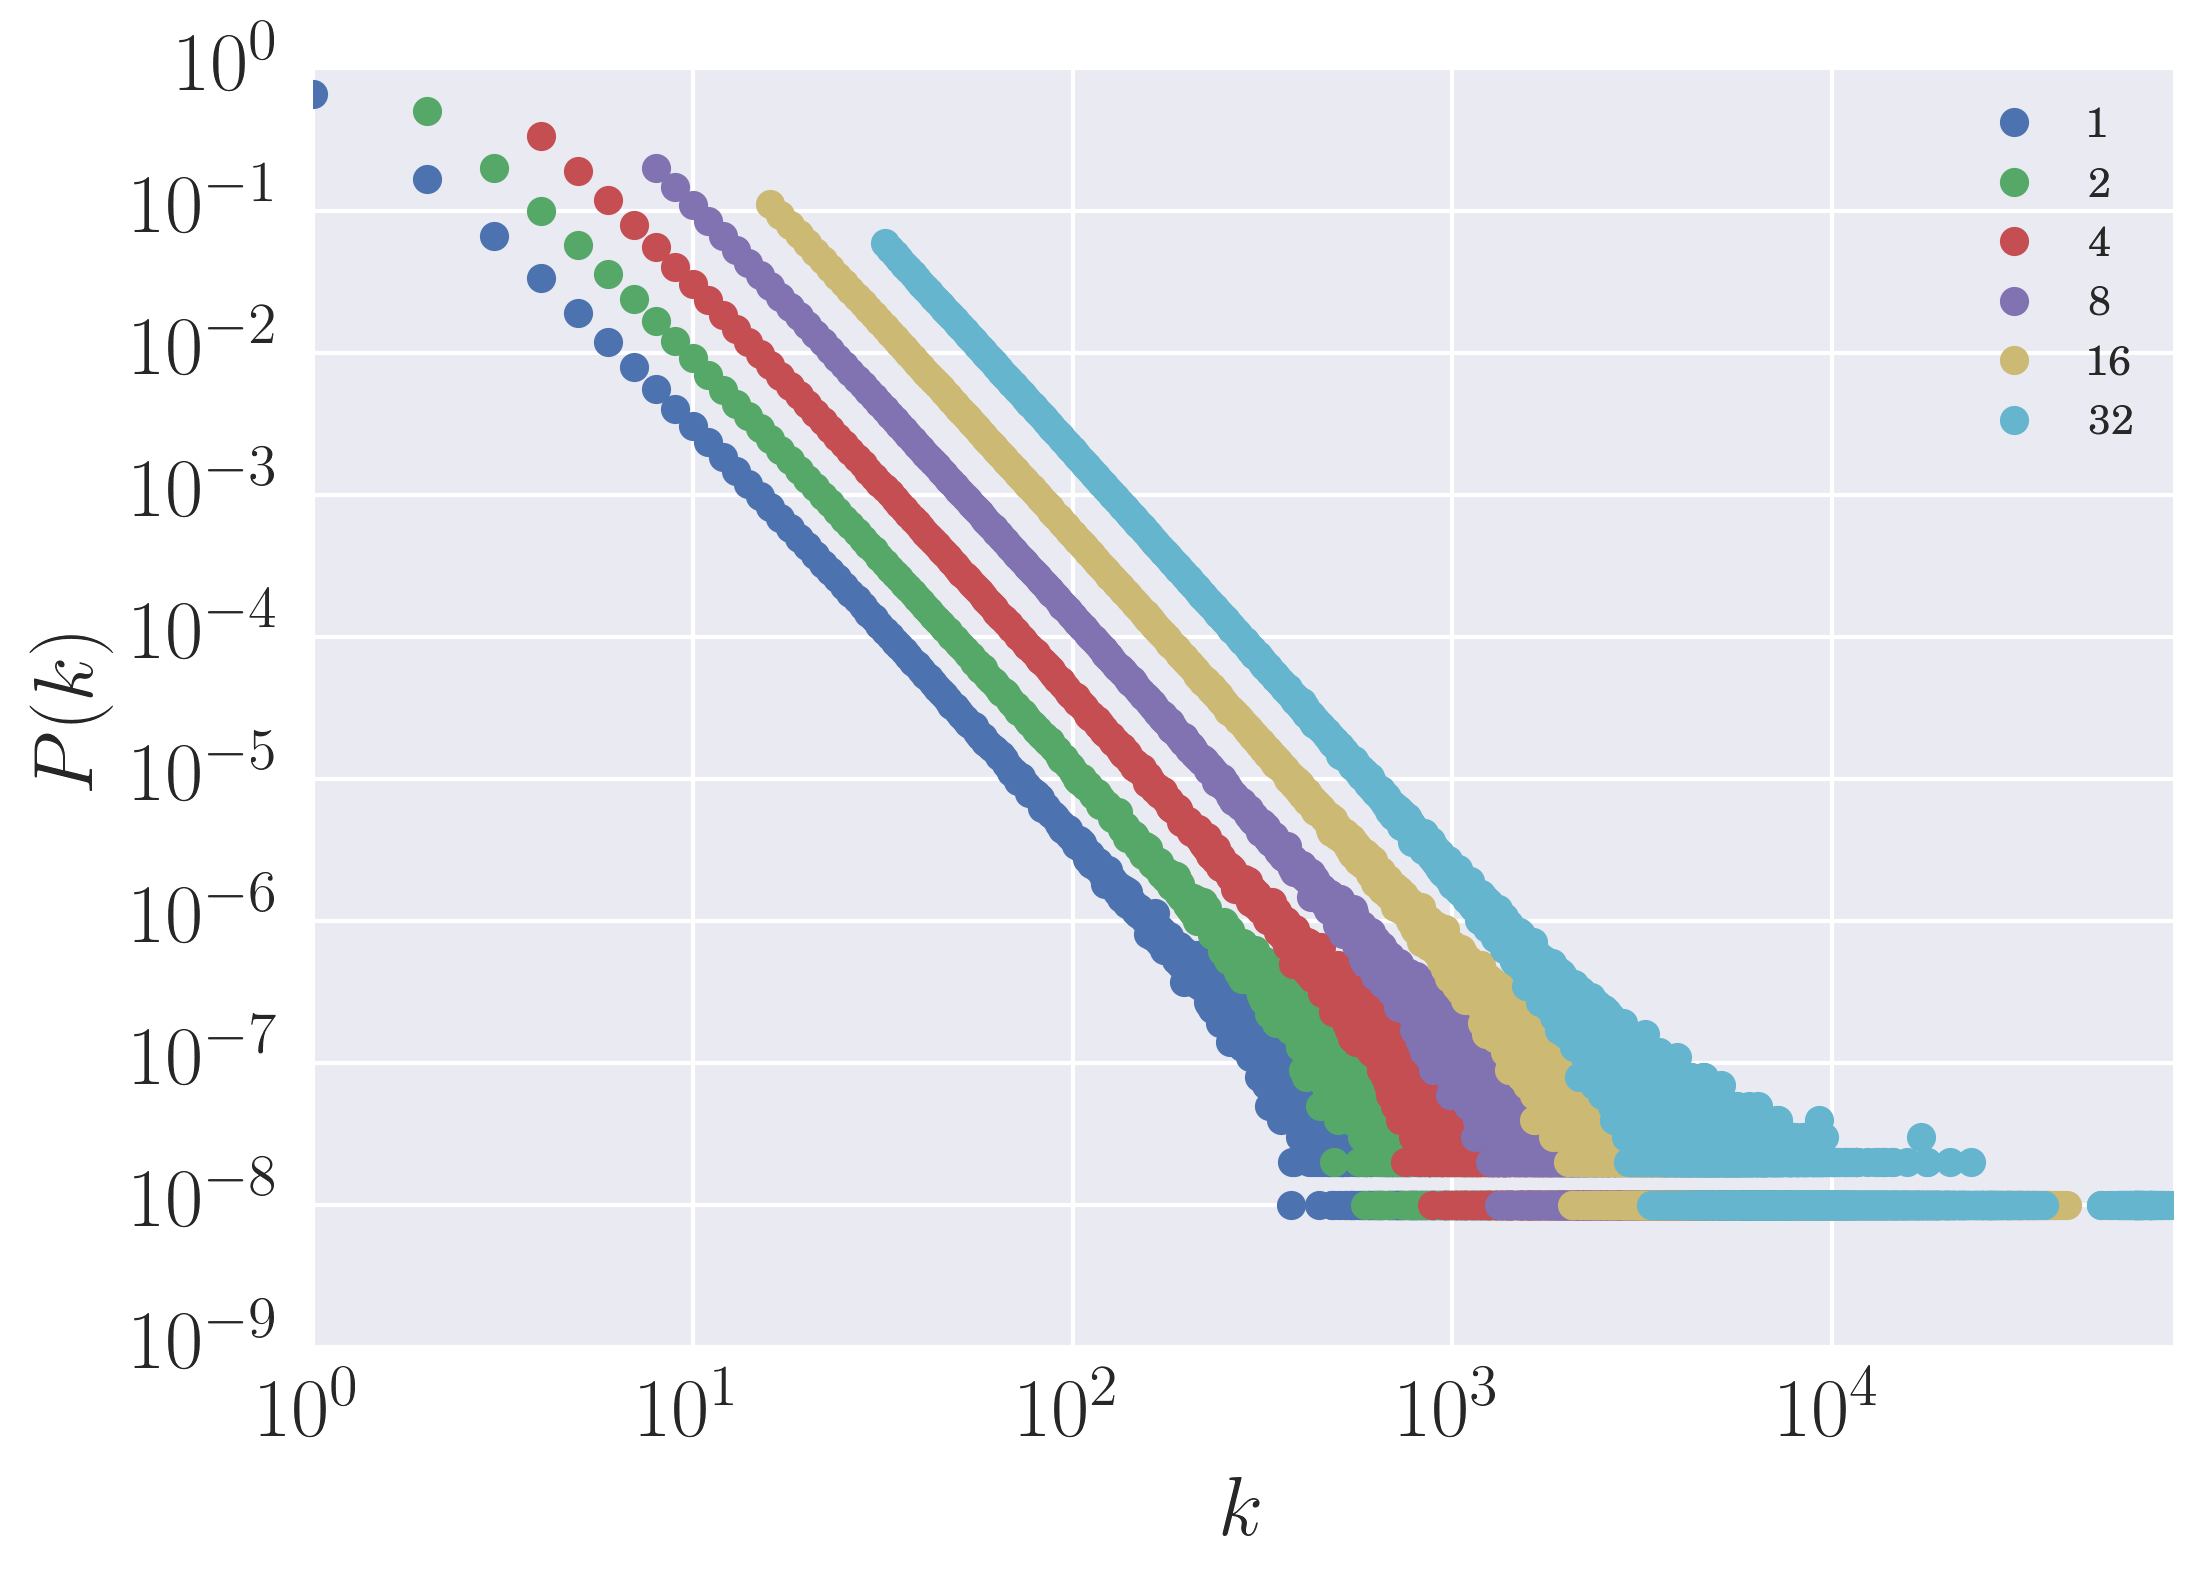
\includegraphics[height=0.5\linewidth]{img/pa-fixed-n-degree-dist}
    \caption{Raw degree distribution averaged over 100 runs for $m = 1, 2, 4, 8, 16, 32$. A noisy tail can still be seen at large $k$ due to finite sized effects. }
    \label{fig:pa-fixed-n-degree-dist}
\end{figure}

Visually, as can be seen from \autoref{fig:pa-fixed-n-logbin}, the numerical results seem to agree with the theoretical model after log-binning, until finite sized effects begin to kick in at large $k$. Alternatively, we can look at the complementary cumulative distribution function (ccdf) to observe the behaviour of the fat tail more clearly. This is shown in \autoref{fig:ccdf}. We can see that near the fat tail, the numerical ccdf goes slightly higher than the theoretical, before falling off. This is consistent across different $m$ values.

\begin{figure}
    \centering
    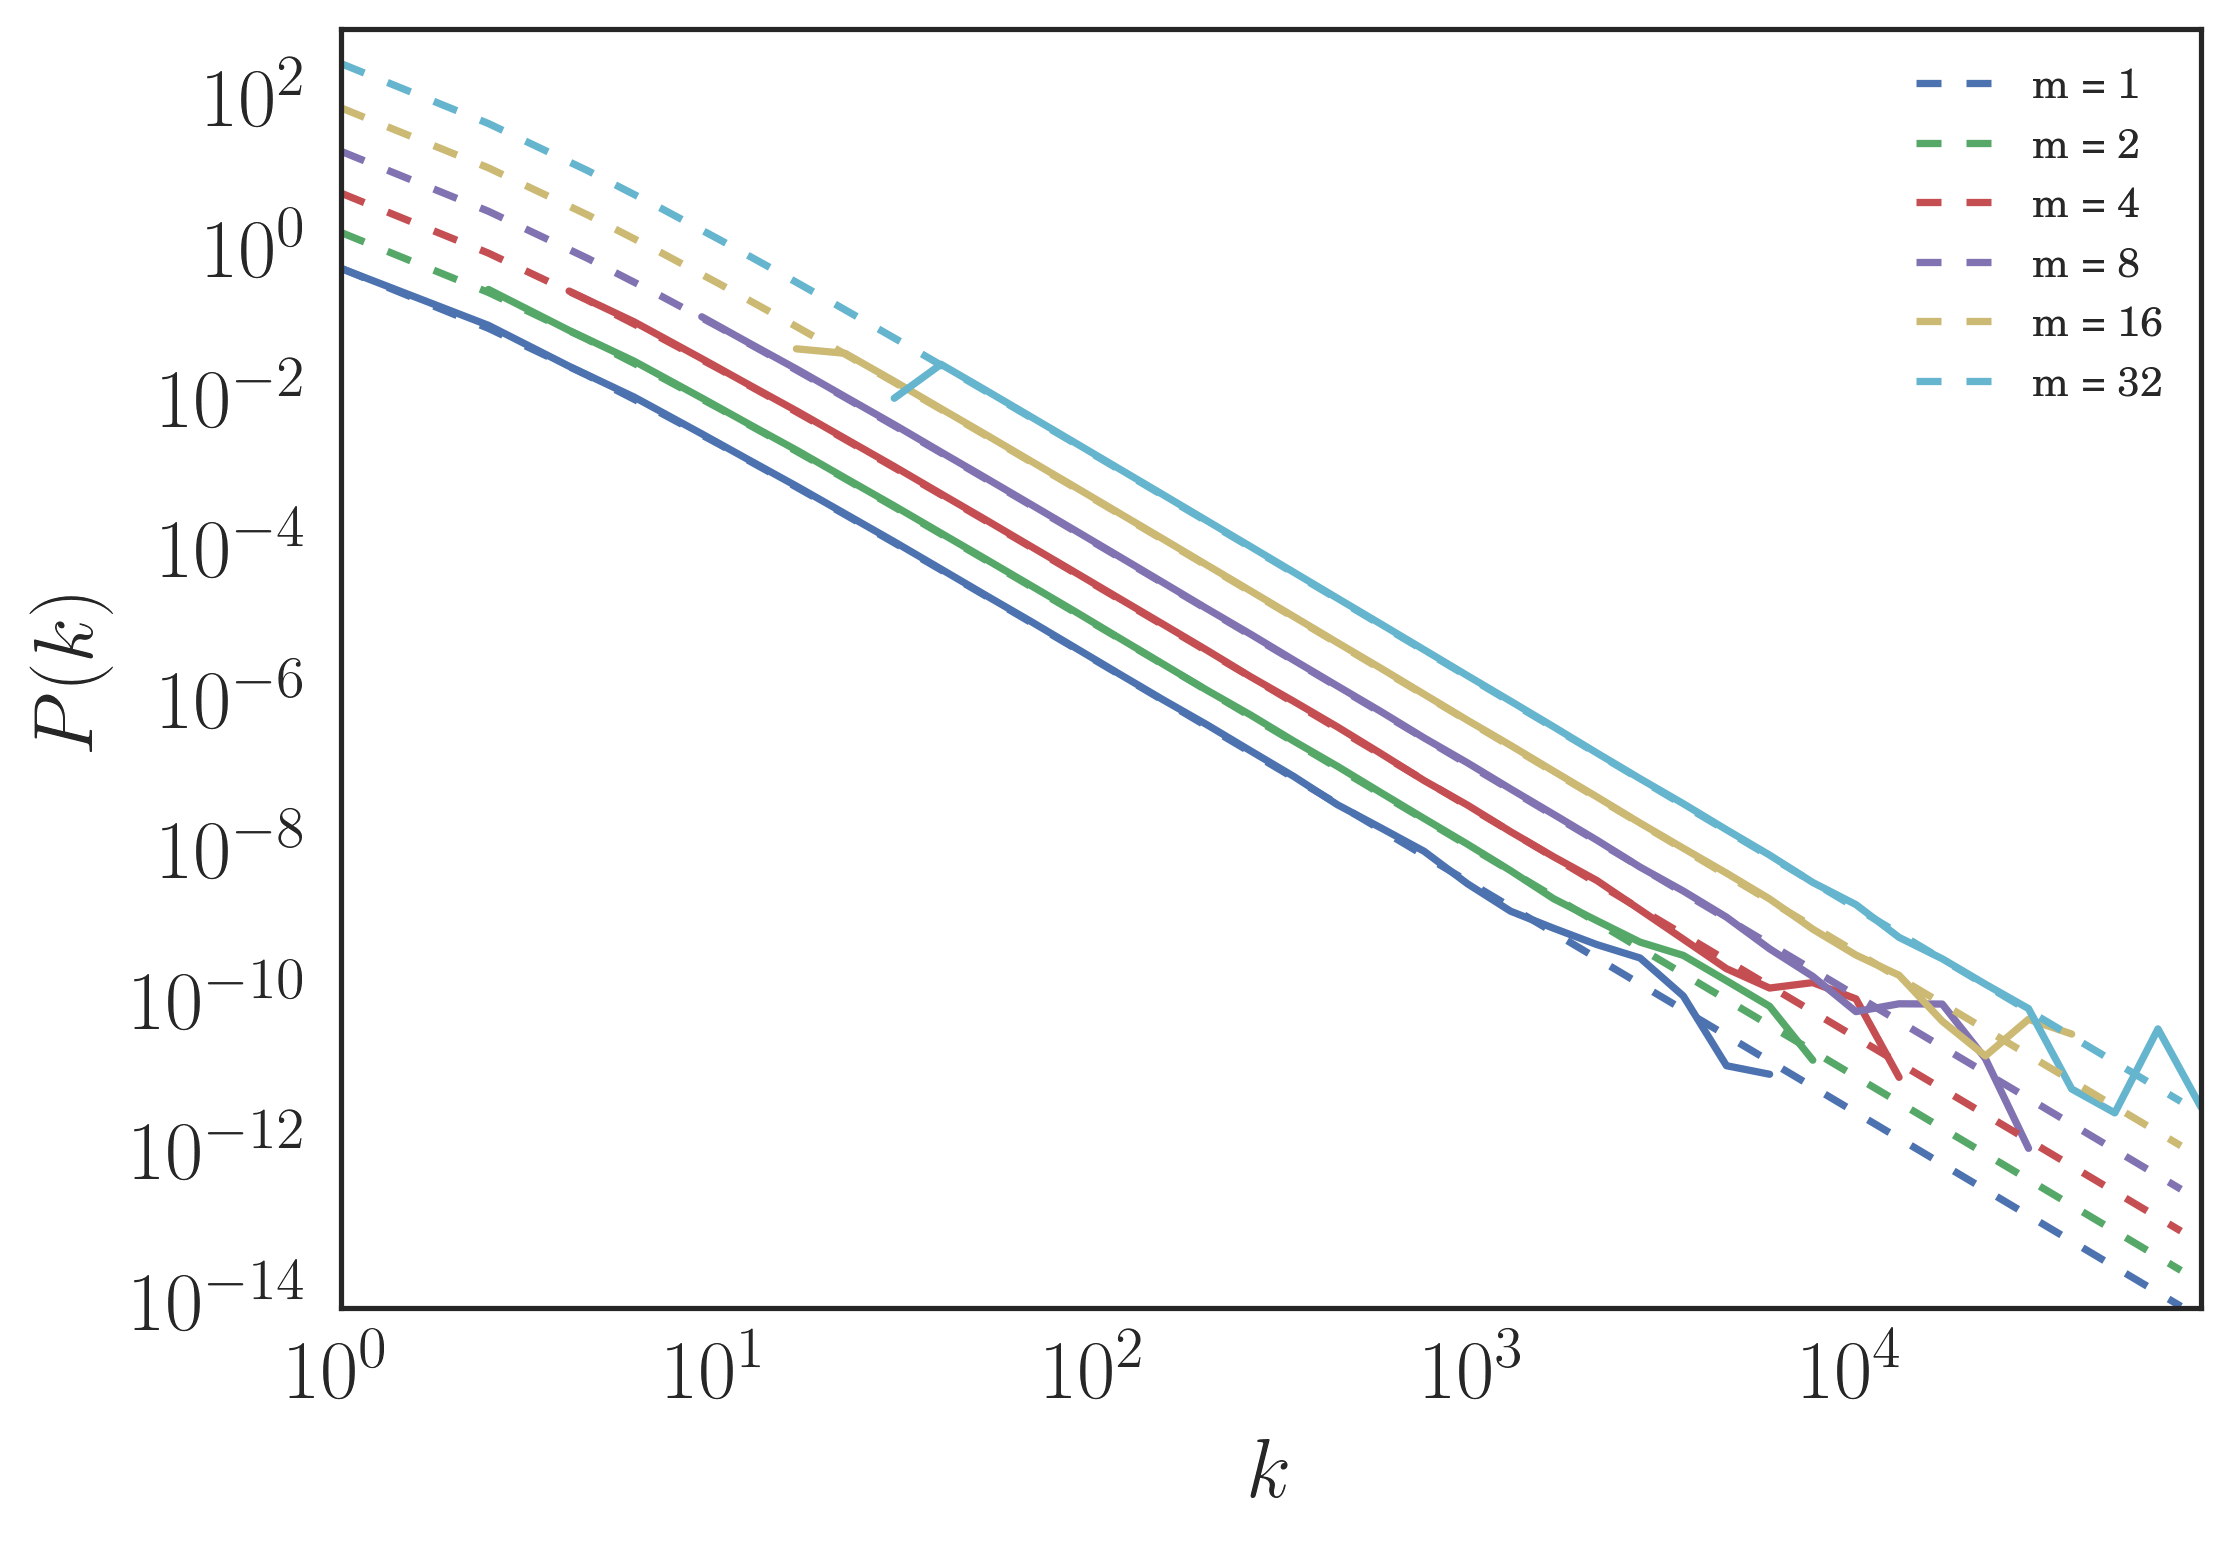
\includegraphics[height=0.5\linewidth]{img/pa-fixed-n-logbin}
    \caption{The solid lines show log-binned degree distributions for $m = 1, 2, 4, 8, 16, 32$. The dashed lines show the values predicted by the theoretical model. There is good agreement for small $k$ finite sized effects kick in. }
    \label{fig:pa-fixed-n-logbin}
\end{figure}

\begin{figure}
    \centering
    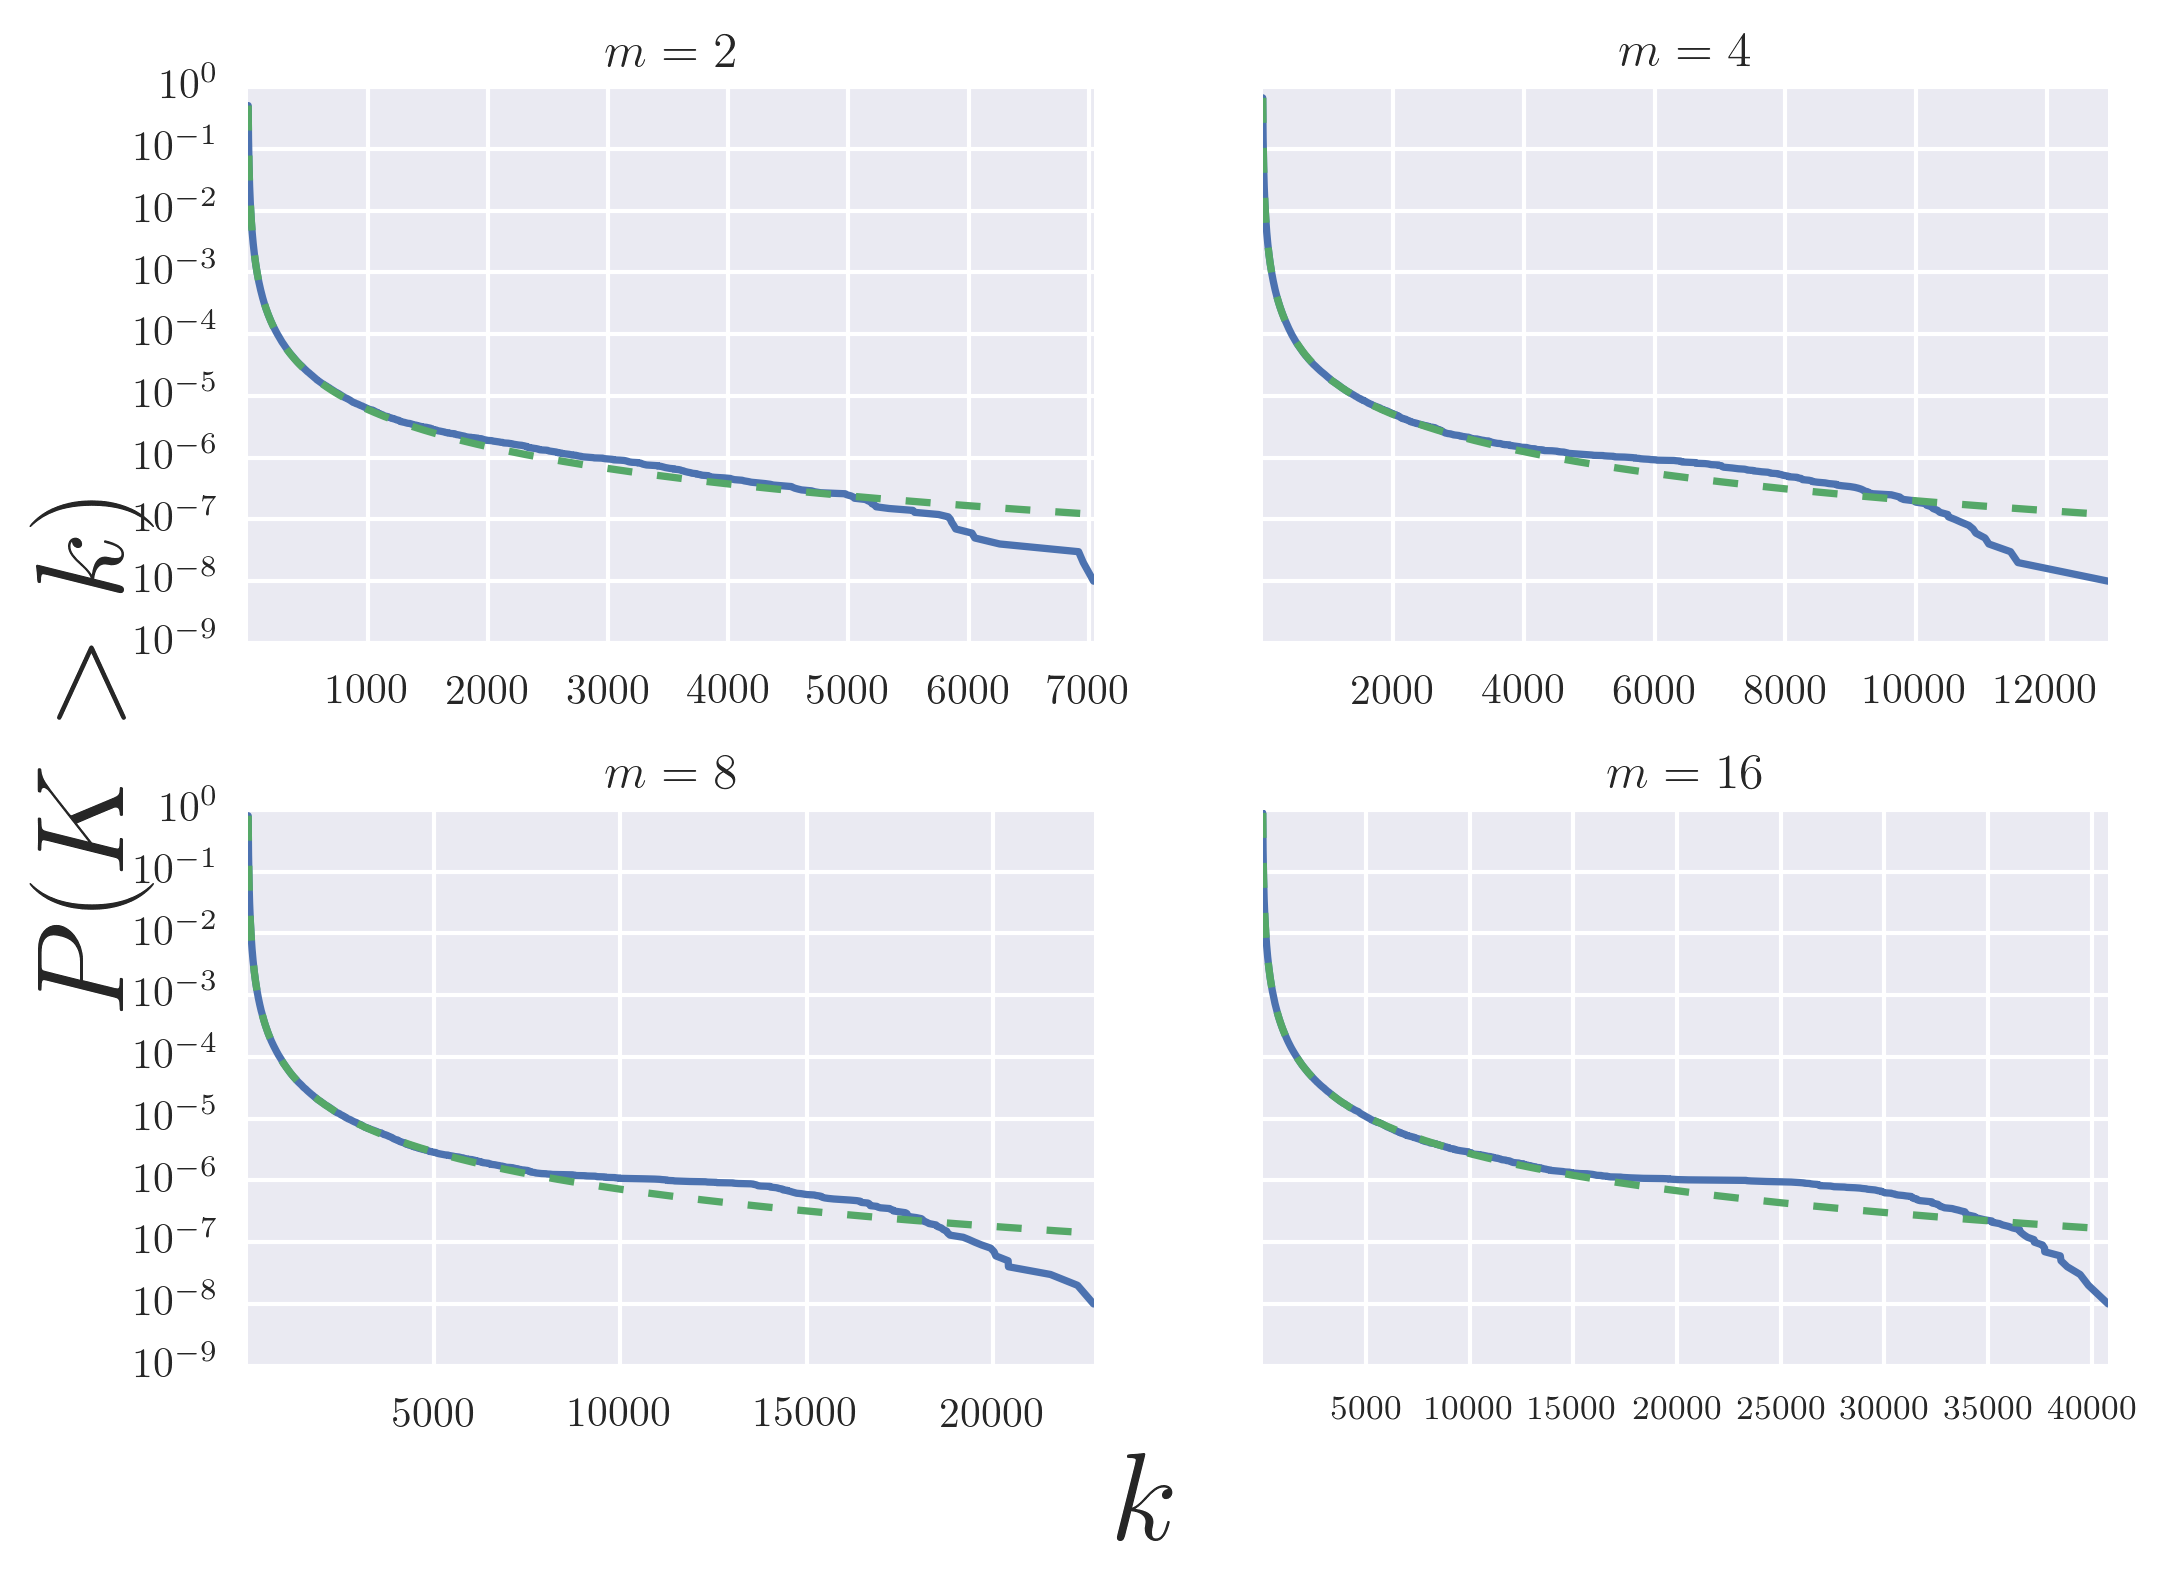
\includegraphics[height=0.7\linewidth]{img/ccdf}
    \caption{CCDF of $m=2, 4, 8, 16$, where the solid line is the numerical CCDF and the dotted line is the CCDF predicted by theory.}
    \label{fig:ccdf}
\end{figure}

A Kolmogorov-Smirnov (KS) test was used to quantify the goodness-of-fit between theory and numerical results. It is a non-parametric test that measures how far apart two distributions are, and it returns a KS-statistic that can be converted into a p-value. A smaller KS-statistic implies that the numerical data and theoretical distribution are more similar and that differences between data and model may be attributed to statistical differences, while a large KS-statistic that the model is unlikely to have been the generating function for the data. 

The table below shows the results of the KS test on $m = 1$ to $m=32$:

\begin{center}
\begin{tabular}{ c | c }
 m &  KS-statistic \\ 
 \hline
 1 & 0.000414 \\  
 2 & 0.000978 \\
 4 & 0.000744 \\
 8 & 0.000662 \\
 16 & 0.001002 \\
 32 & 0.001132 \\  
\end{tabular}
\label{table:ks-test}
\end{center}

However, these values are meaningless unless we know what kind of deviation from theoretical is considered acceptable, and at what value we should reject the null hypothesis. To answer that, we generate synthetic datasets governed by the theoretical distribution in \autoref{eq:p-infinity-solution} to measure how far they fluctuate from the reference theoretical distribution in a similar way as described by \citet{Clauset2009}, and compare the results with the simulated data. 

The synthetic datasets were generated with a lower bound of $m$ and an upper bound given by the maximum degree in the simulated dataset. If the simulated data is much further from the theoretical distribution than the typical synthetic data, then we would have grounds to reject the null hypothesis. 

For each of the synthetic datasets, we compare it to the theoretical distribution and calculate its KS-statistic. Then we define our $p$-value as the fraction of the time the resulting statistic is larger than the value for the numerical data. We can then reject the null hypothesis if $p \leq 0.1$ \citep{Clauset2009}, that is, if there is a 1 in 10 probability or less that we would, by chance, get data that agree as poorly with the model as the current data. 

Another issue to consider is the number of synthetic datasets to generate. Again, \citet{Clauset2009} suggests a useful rule: to have p-values accurate to within about $\epsilon$, we need at least $\frac{1}{4}\epsilon^{-2}$ datasets. In this project, 100 datasets were generated for each $m$, to get an accuracy of about $0.05$. 

The resulting p-values are given in the table below:
\begin{center}
\begin{tabular}{ c | c }
 m &  p-value\\ 
 \hline
 1 & 0.71 \\  
 2 & 0.45 \\
 4 & 0.50 \\
 8 & 0.58 \\
 16 & 0.71 \\
 32 & 0.46 \\  
\end{tabular}
\captionof{table}{The list of $p$-values for each $m$ for preferential attachment when compared with synthetic datasets.}
\label{table:ks-test-all}
\end{center}

Since the $p$-values for each $m$ are all larger than $0.1$, we can say it is plausible that the numerical data was drawn from the theoretical distribution. 

A point to note is that the KS test is used for continuous distributions, while our degree distribution is discrete. However, it was assumed that for large $N$, there will be values spanning a large range of $k$, hence the change in $k$ can be considered small, and the distribution can be approximated as a continuous distribution. 

A chi-squared test was also considered. The chi-squared test is a categorical test, suitable for discrete distributions, however, the test becomes invalid when the observed or expected frequencies for each category is too small, with a typical rule being that the frequencies should be at least 5 \citep{Lawrence1997}. In our numerical data, there many large values of $k$ that only appeared once, and hence this test was determined to be not suitable. 

\subsection{Largest expected degree: Theory}
The finite size of the system imposes a structural cutoff on the largest expected degree. For scale free networks, \citet{Aiello2001a} defined the maximum degree to be approximately the value above which there is less than one vertex of that degree in the graph on average, that is, $N \sum_{k = k_1}^\infty p_\infty(k) = 1$. 

Generally, it is shown \citep{Boguna2004} that for a scale free network with $p_{\infty}(k) \propto k^{\gamma}$, the largest expected degree will be

\begin{equation}
	k_1(N) \sim N^{1 / (\gamma -1)}.
	\label{eq:largest-expected-degree-research}
\end{equation}
Starting with the equation 

\begin{equation}
	N \sum_{k=k_1}^\infty p_{\infty}(k) = 1, 
	\label{eq:largest-expected-degree-criteria}
\end{equation}
we can see that this is almost identical to \autoref{eq:normalization-criteria}, just with a different factor and lower limit. Hence we have 
\begin{equation}
	2m(m+1) \frac{1}{2k_1(k_1+1)} = \frac{1}{N}.
	\label{eq:largest-expected-degree-derivation}
\end{equation}
We can then rearrange this to give us an expression for $k_1$:
\begin{equation}
	k_1 = \frac{-1 + \sqrt{1 + 4Nm(m+1)}}{2}
	\label{eq:pa-k1-expression}
\end{equation}
where the other negative solution is rejected as it is unphysical, and confirming that verifying that $k \propto N^{0.5}$. 

\subsubsection{Numerical analysis: Largest expected degree}\label{subsection:pa-numerical-largest-degree}

As can be seen from the \autoref{fig:pa-numerical-theoretical-k1}, the numerical value seems to be consistently slightly lower than the theoretical $k_1$ values. This is reasonable since numerical simulations are for finite $N$, and hence there will be an upper limit to the possible degrees that a vertex can take, while in the theoretical derivation, there is no upper limit to the possible values of $k$ that a vertex can have. By looking at the ratios of $ k_1 \text{(numerical)} / k_1 \text{(theoretical)} $ as shown in \autoref{table:pa-numerical-theoretical-ratio}, we can see that deviations are generally constant. 

By repeating numerical simulations for 100 times, we can estimate the error on $k_1$ by calculating the standard deviation for the sample and using the following formula to estimate population standard deviation:

\begin{equation}
	\sigma = \sqrt{\frac{1}{n} \sum_{i=1}^n (k_{1, i} - \bar{k}_1)^2}
	\label{eq:population-std}
\end{equation}
where $n$ is the number of repeats. In this case, $n = 100$. 

The values can be seen in \autoref{table:pa-numerical-theoretical-ratio}, 


\begin{figure}
    \centering
    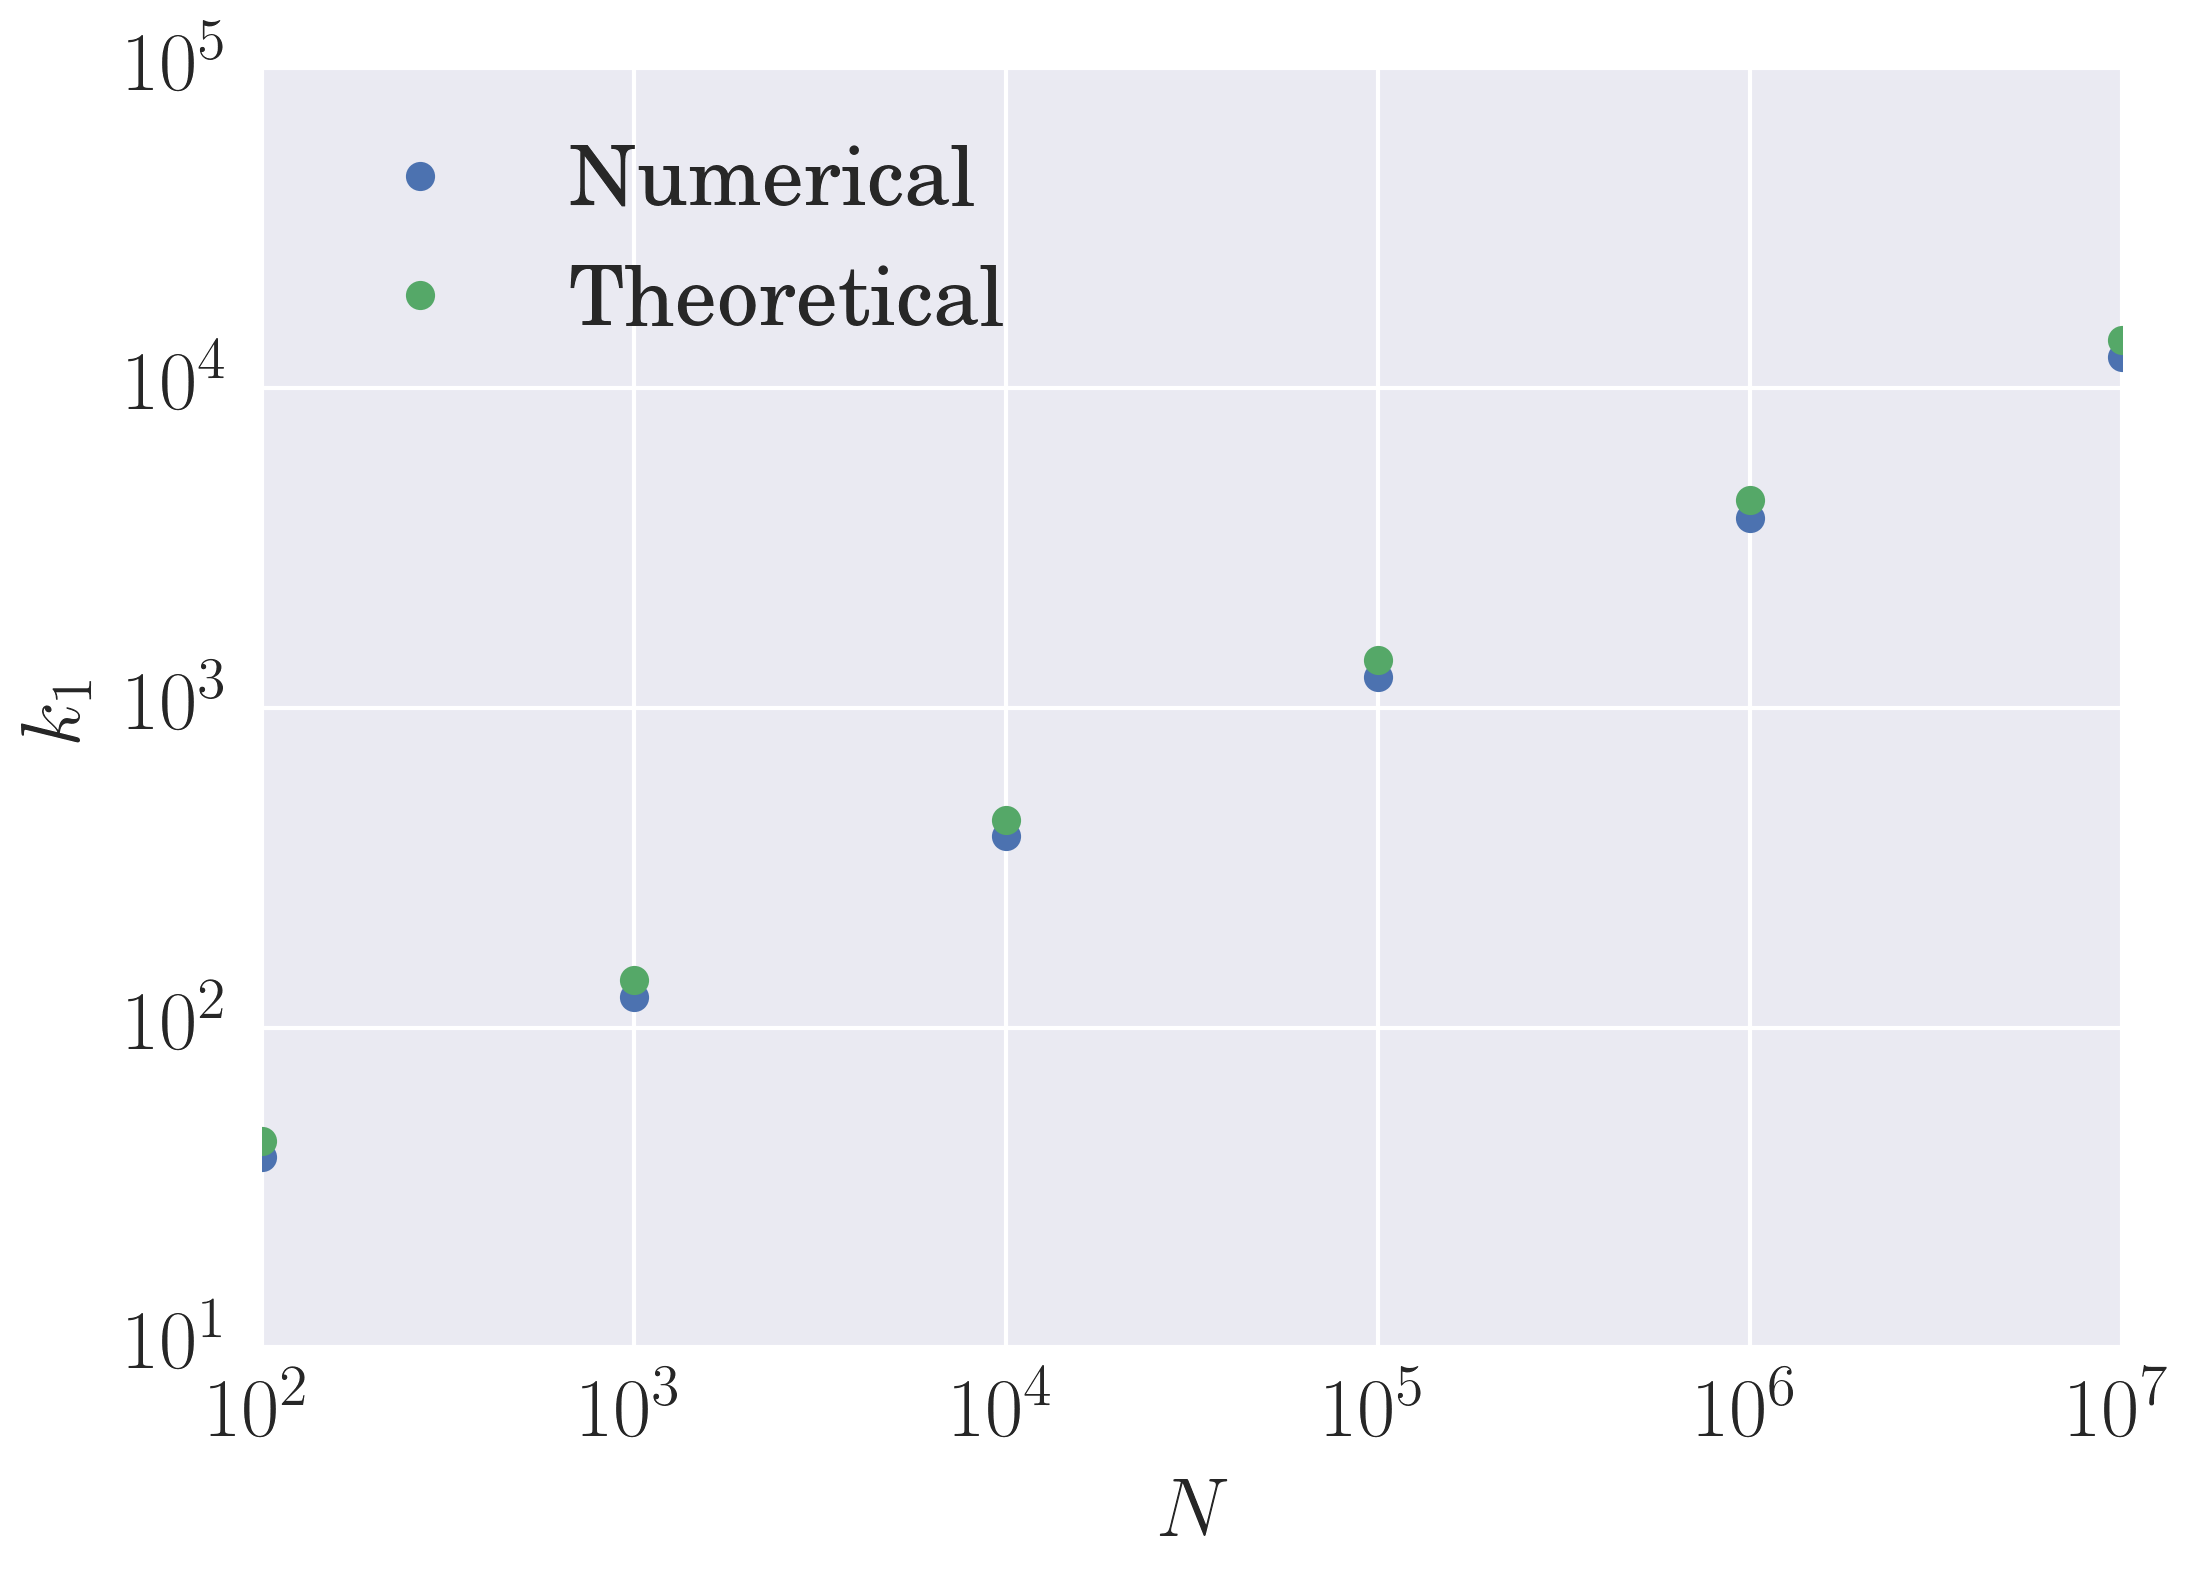
\includegraphics[height=0.5\linewidth]{img/pa-numerical-theoretical-k1}
    \caption{This shows the difference in $k_1$ for different values of $N$ ranging from $100$ to $10^7$ for preferential attachment. There is a constant offset of the numerical values from the theoretical, indicating a systematic bias instead of statistical fluctuations. }
    \label{fig:pa-numerical-theoretical-k1}
\end{figure}

\begin{center}
\begin{tabular}{ ||c | c | c | c ||}
\hline
N & $k_1^{\text{theory}}$ & $k_1^{\text{numerical}}$ & $k_1^{\text{numerical}} / k_1^{\text{theory}} $\\ 
\hline
$10^2$ & 45    & 39.3  $\pm$ 0.1 & 0.889 \\  
$10^3$ & 141   & 124.9 $\pm$ 0.3 & 0.886 \\
$10^4$ & 447   & 396   $\pm$  1  & 0.887 \\
$10^5$ & 1414  & 1248  $\pm$  3  & 0.883 \\
$10^6$ & 4472  & 3924  $\pm$  9  & 0.878 \\
$10^7$ & 14142 & 12558 $\pm$ 30  & 0.888 \\  
\hline
\end{tabular}
\label{table:pa-numerical-theoretical-ratio}
\captionof{table}{This table shows the theoretical and numerical values for the largest expected degree as defined in \autoref{eq:pa-k1-expression} for preferential attachment. The errors on $k_1$ are rounded off to 1 significant figure. }
\end{center}


To produce a data collapse, we need to find the function $f$ such that 

\begin{equation}
	p_N(k) = f(k) \mathcal{G}\left ( k / k_1 \right )
	\label{eq:data-collapse}
\end{equation}

To find $f(k)$, we know that in the limit of $N \rightarrow \infty$, $p$ must have no dependence on $L$, and in the large $N$ limit, $p_N(k) = f(k)$ which is just $p_{\infty}(k)$. This implies 
\begin{equation}
	\frac{p_N(k)}{p_{\infty}(k)} = G \left ( k / k_1 \right )
\end{equation}
which means that plotting $p_N(k) / p_{\infty}(k)$ against $k / k_1$ will produce a data collapse, as shown in \autoref{fig:pa-data-collapse}. 

\begin{figure}
    \centering
    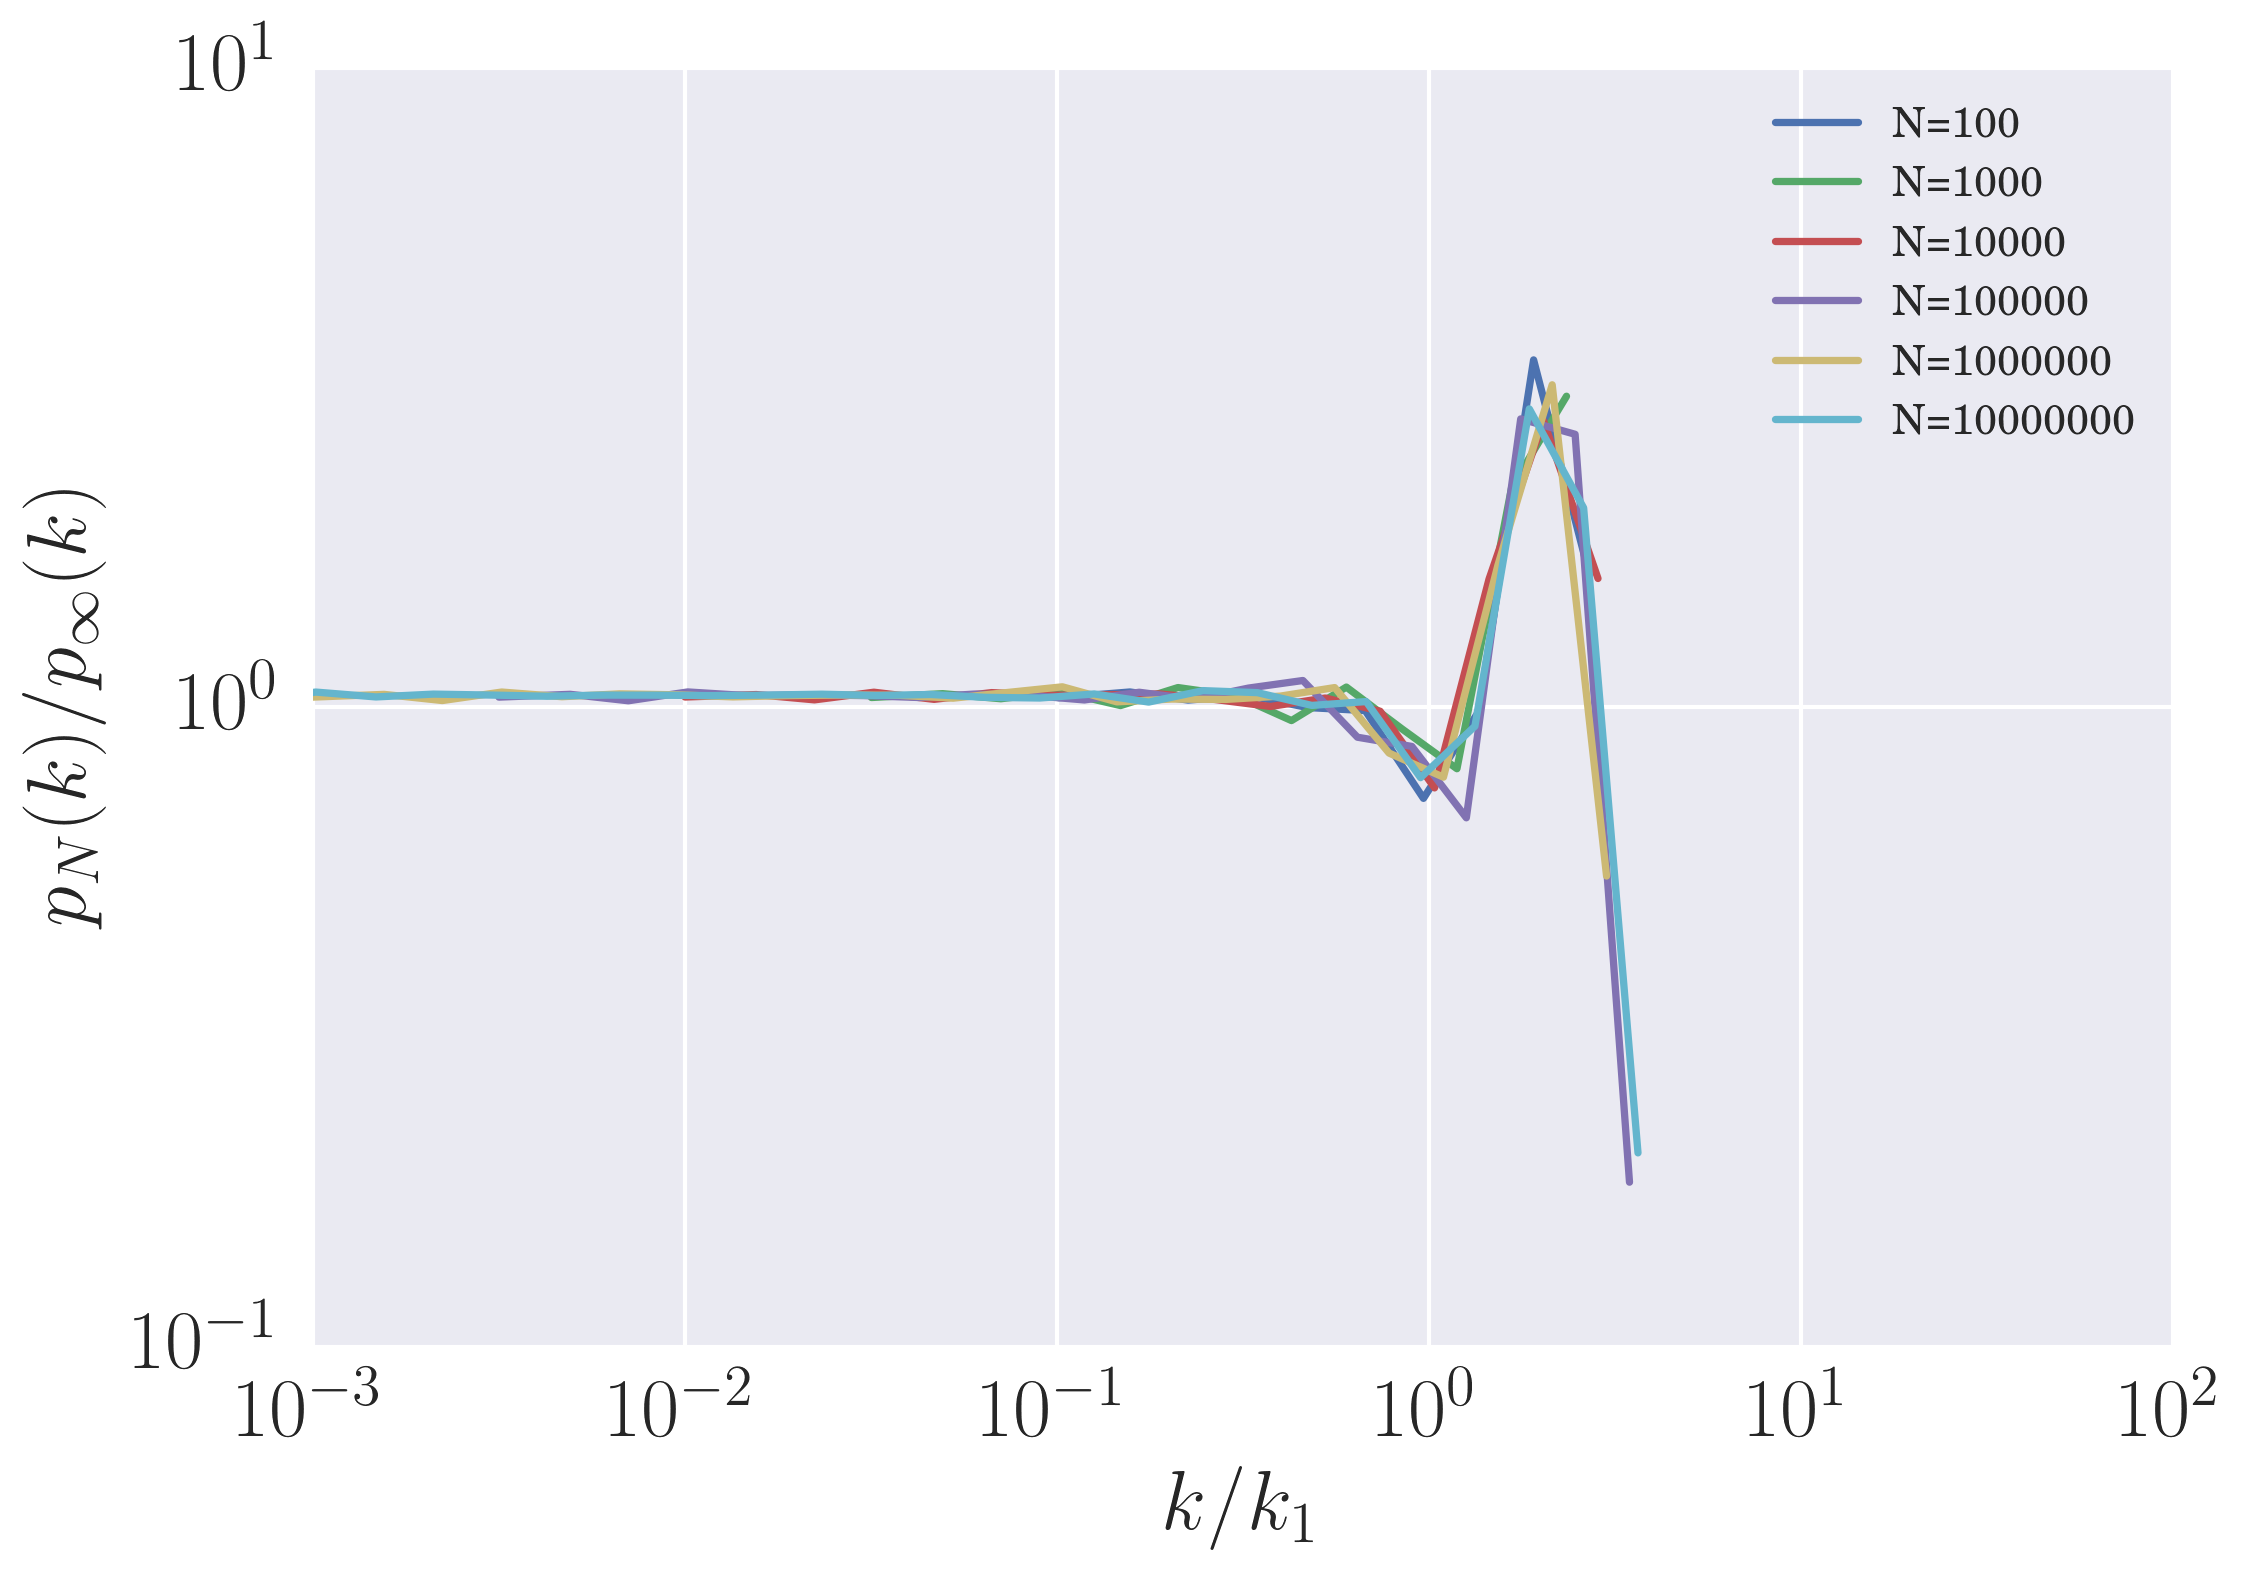
\includegraphics[height=0.5\linewidth]{img/pa-data-collapse}
    \caption{Data collapse of the degree distribution for networks of size $N=10^2, 10^3, 10^4, 10^5, 10^6, 10^7$}
    \label{fig:pa-data-collapse}
\end{figure}
%!TEX root = ../main.tex
\section{Pure random attachment}\label{section:pure-random-attachment}

\subsection{Degree distribution: Theory}
The pure random attachment model can be seen as a limiting case of the BA model. In this model, all existing vertices are chosen with equal probability, i.e. $\Pi = \Pi_{rnd} \propto 1$. This preserves growth but removes preferential attachment. 

Similar to the previous section, we start from the master equation in \autoref{eq:master}, and instead of $\Pi = k/ 2E(t)$ as in preferential attachment, we use $\Pi_{rnd} = 1 / N(t)$. Again, we consider the long-time ansatz $n(k, t) \rightarrow N(t) p_{\infty}(k)$. Substituting these terms into \autoref{eq:master}, we have

\begin{equation}
	p_{\infty}(k) = m p_{\infty}(k-1) - m p_{\infty}(k) + \delta_{k, m}. 
	\label{eq:ra-degree-distribution-p-infinity}
\end{equation}

Considering the case of $k > m$, we obtain the recurrence relation
\begin{equation}
	p_{\infty}(k) = \left ( \frac{m}{m+1} \right ) p_{\infty}(k-1)=...= \left ( \frac{m}{m+1} \right )^{k-m} p_{\infty}(m)
	\label{eq:ra-degree-recurrence-relation}
\end{equation}

Now we consider $k=m$. Substituting $k=m$ into \autoref{eq:ra-degree-distribution-p-infinity} and remembering that $p_{\infty}(k < m) = 0$, we get
\begin{equation}
	p_{\infty}(m) = -mp_{\infty} + 1, 
	\label{eq:ra-degree-k-equal-m}
\end{equation}
giving us 
\begin{equation}
	p_{\infty}(m) = \frac{1}{m+1}. 
	\label{eq:ra-degree-p-infinity-m}
\end{equation}

Combining this result with \autoref{eq:ra-degree-recurrence-relation}, we get the following formula for $p_{\infty}(k)$:
\begin{equation}
	p_{\infty}(k) = \frac{1}{m+1} \left ( \frac{m}{m+1}\right )^{k-m}.
	\label{eq:p-infinity-solution-ra}
\end{equation}

For normalization, we need to check that 
\begin{equation}
	\sum_{k=m}^{\infty}p_{\infty}(k) = \frac{1}{m+1} \sum_{k=m}^{\infty} \left ( \frac{m}{m+1}\right )^{k-m} = 1.
	\label{eq:ra-check-normalization}
\end{equation}
The terms in the summation form a converging geometric series, with the starting term being zero and common ratio being $m / (m+1)$. Hence we have 
\begin{equation}
	\sum_{k=m}^{\infty} \left ( \frac{m}{m+1} \right )^{k-m} = \frac{1}{1 - [m / (m+1)]}. 
	\label{eq:ra-geom-series}
\end{equation}

By substituting this back into the \autoref{eq:ra-check-normalization}, we can see that normalization is satisfied. 

As we can see from \autoref{eq:p-infinity-solution-ra}, the resulting degree distribution in this limit is geometric \citep{Pekoz2013}, indicating that growth alone is not sufficient to produce a scale free structure. 

\subsection{Degree distribution: Numerical analysis}\label{subsection:ra-numerical-analysis}
Numerical simulations confirmed that growth alone is not sufficient to produce a scale free structure. \autoref{fig:ra-fixed-n-degree-dist} shows the raw degree distribution of numerical simulations for $N=10^6$ and different values of $m$. The fat tail was reduced by taking the average of multiple simulations. Already, we can see that it does not follow a power law. After log binning, it follows the theoretical geometric simulation very well for small $k$, as can be seen in \autoref{fig:ra-fixed-n-logbin}.

\begin{figure}
    \centering
    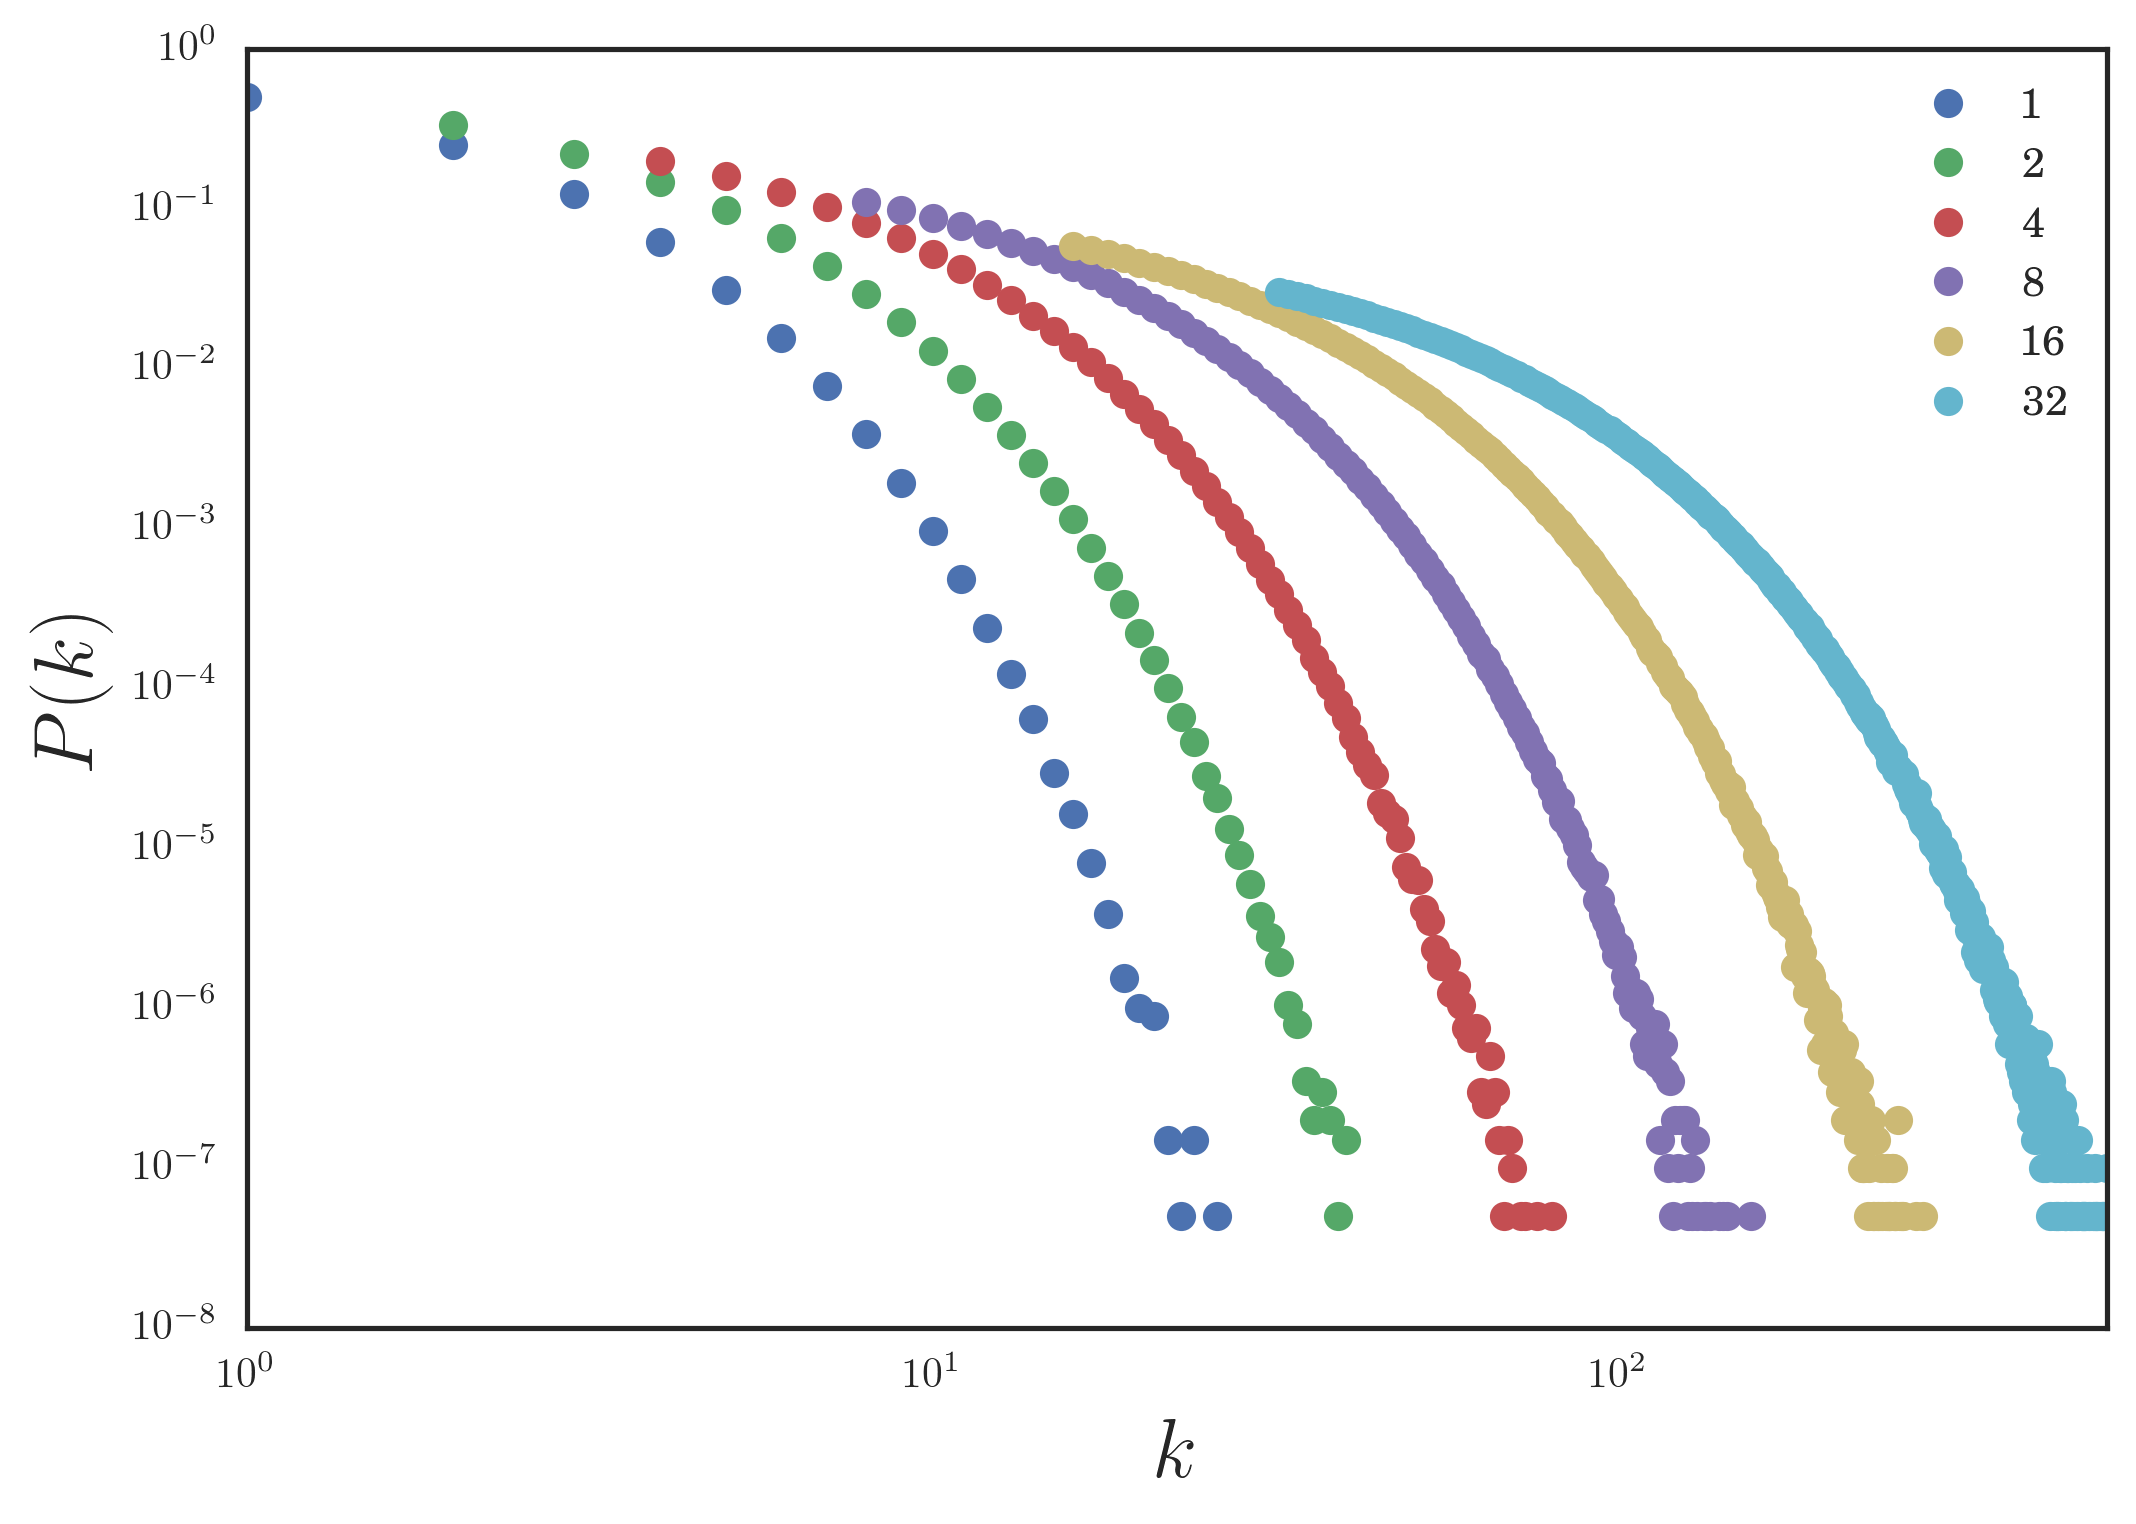
\includegraphics[height=0.5\linewidth]{img/ra-fixed-n-degree-dist}
    \caption{Raw degree distribution for random attachment for $N = 10^6$ and $m = 1, 2, 4, 8, 16, 32$. }
    \label{fig:ra-fixed-n-degree-dist}
\end{figure}

\begin{figure}
    \centering
    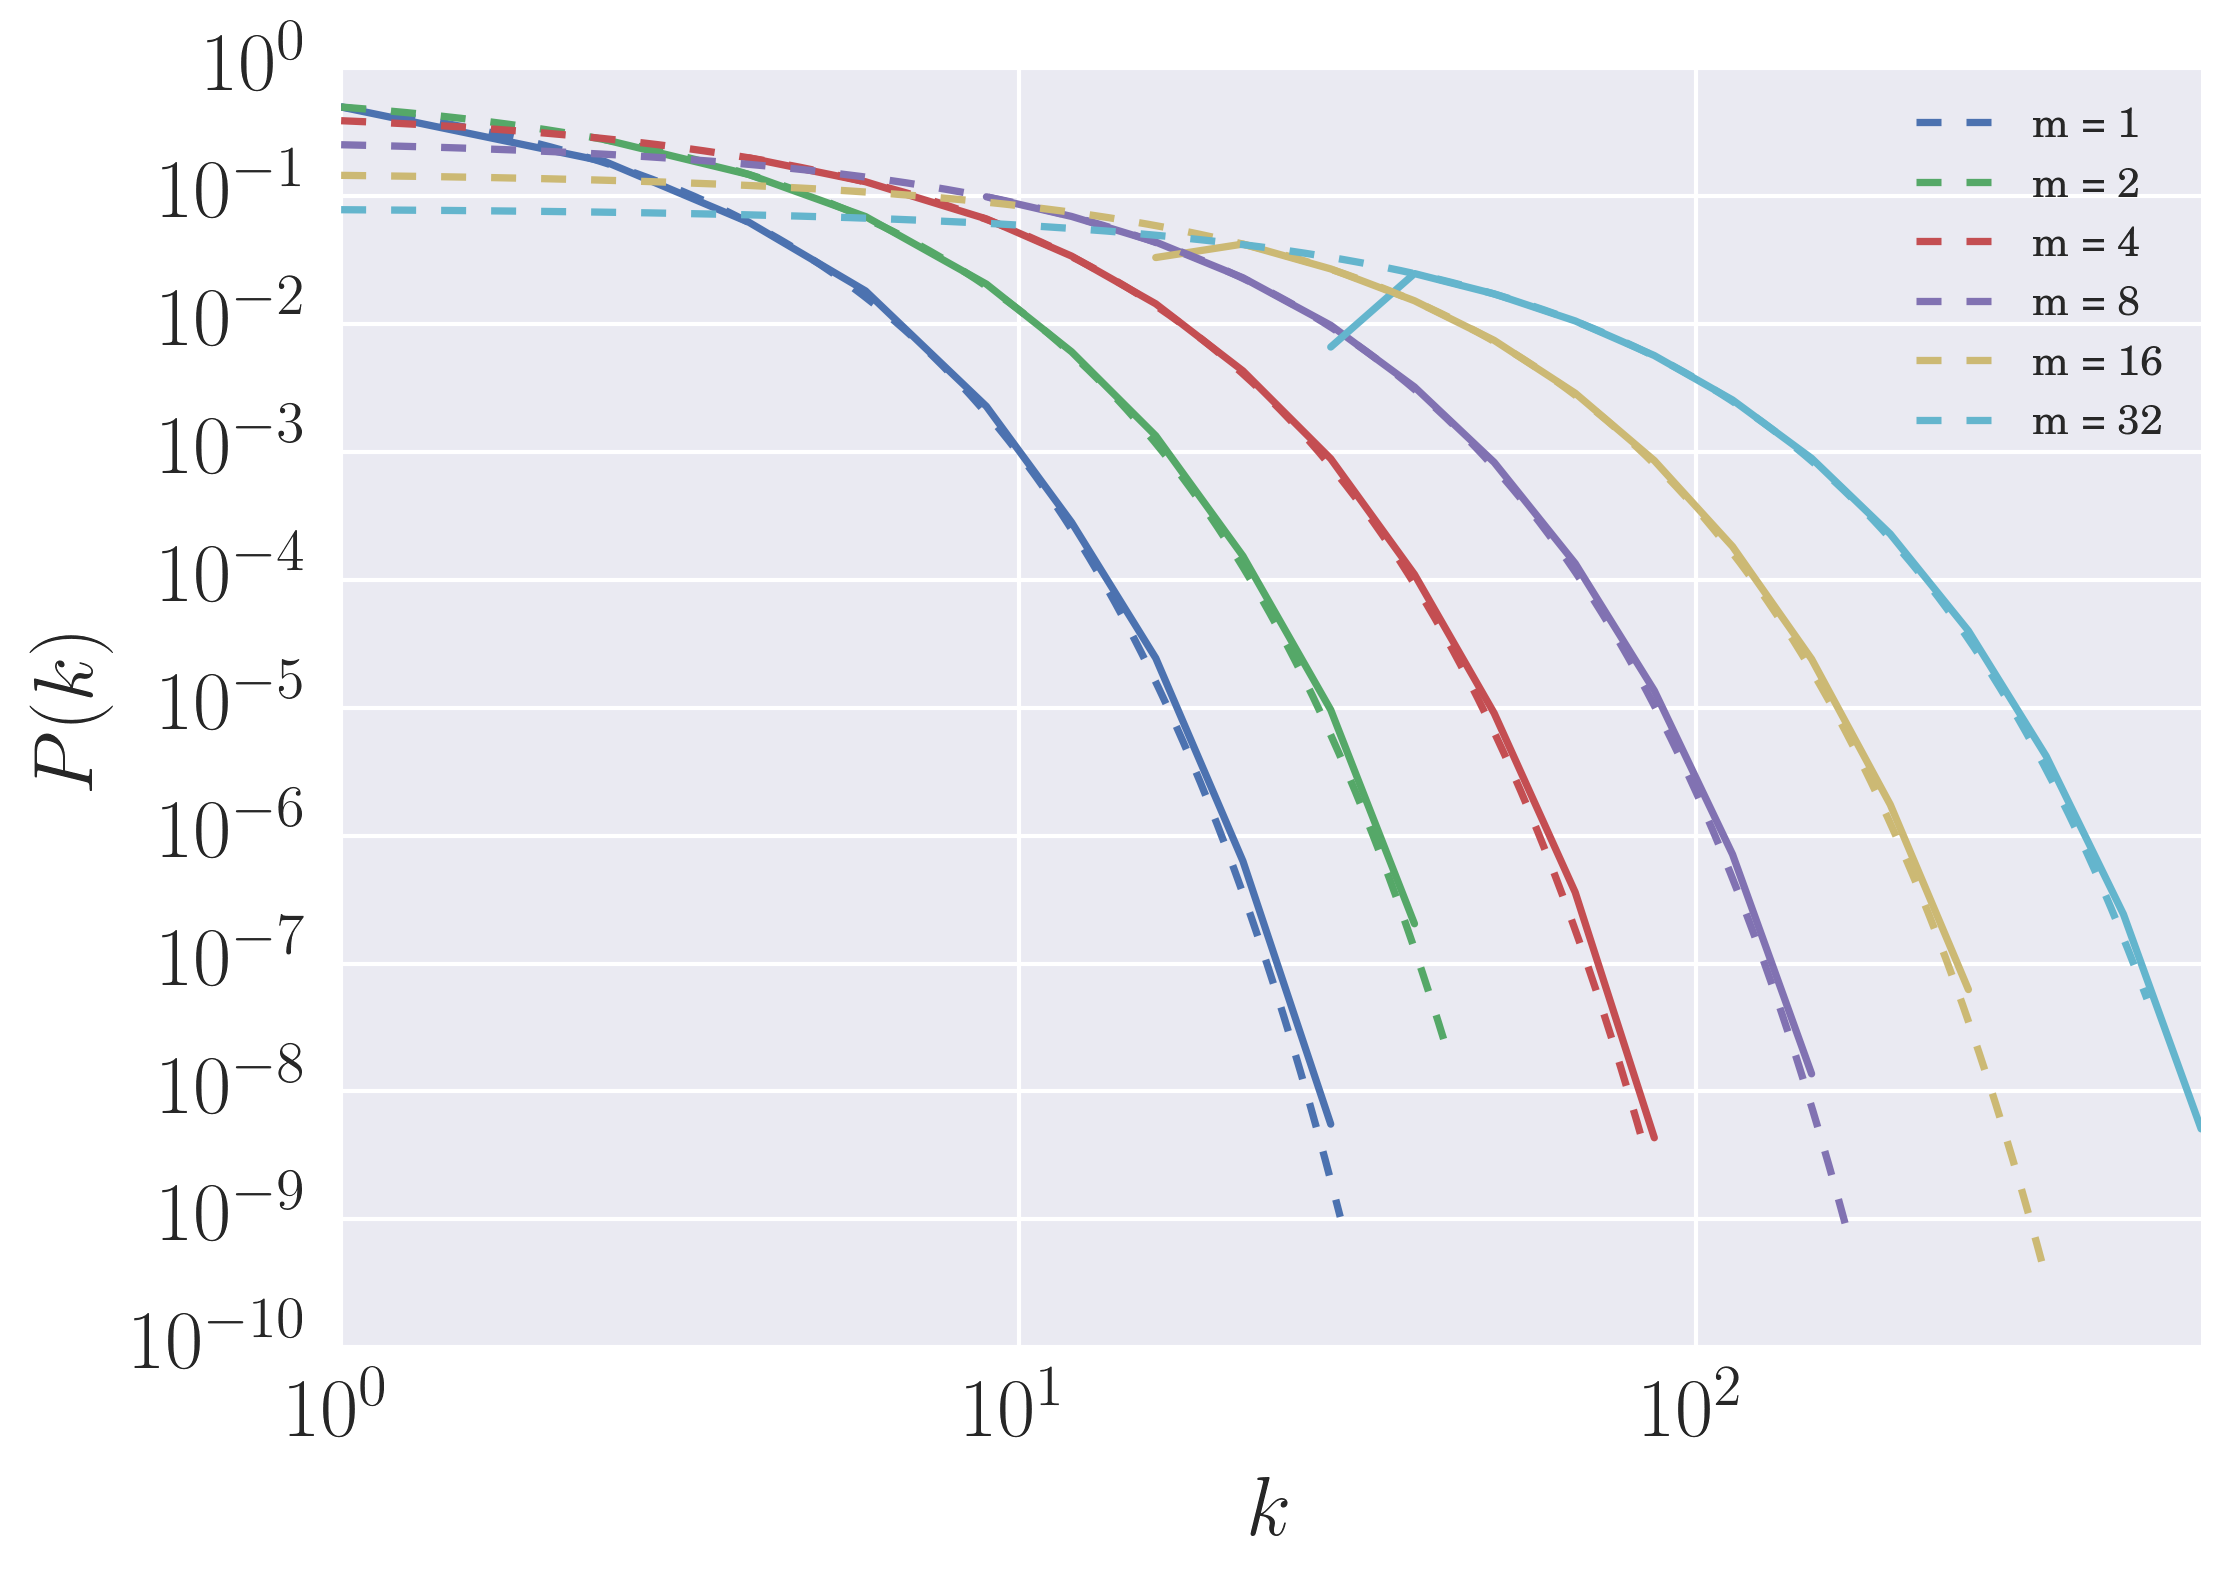
\includegraphics[height=0.5\linewidth]{img/ra-fixed-n-logbin}
    \caption{Data collapse of the degree distribution for networks of size $N=10^2, 10^3, 10^4, 10^5, 10^6, 10^7$}
    \label{fig:ra-fixed-n-logbin}
\end{figure}

Goodness of fit was tested in the same way as in the previous section. When tested against the null hypothesis of a geometric distribution governed by \autoref{eq:p-infinity-solution-ra} p-values obtained are listed below, showing that it is plausible that the simulated data follow the theoretical distribution. While the $p$-values fluctuate between 0.4 and 0.7, they are all safely above the threshold of $0.1$. 

\begin{center}
\begin{tabular}{ c | c }
m & $p$-value \\
\hline
1  & 0.714 \\
2  & 0.446 \\
4  & 0.502 \\
8  & 0.706 \\
16 & 0.456 \\
\end{tabular}
\label{table:ra-ks-test}
\captionof{table}{The list of $p$-values for each $m$ for random attachment when compared with synthetic datasets.}
\end{center}

To demonstrate whether this test is effective, random attachment simulation data was also tested against the power law distribution, and we obtained result of $p = 0$, to an accuracy of $\pm 0.05$, for all $m$. This shows that we can reject the power law hypothesis as expected. 

\subsection{Largest expected degree: Theory}\label{subsection:largest-expected-degree}
Using the same definition from the previous section for largest expected degree, we need

\begin{equation}
	N \sum_{k=k_1}^\infty p_{\infty}(k) = N \sum_{k=k_1}^\infty \frac{1}{m+1} \left (\frac{m}{m+1} \right )^{k-m} = 1.
	\label{eq:largest-expected-degree-ra-criteria}
\end{equation}

Again, the summation is similar to the previous \autoref{eq:ra-geom-series} just with a different lower limit. Applying the geometric series summation formula to the terms in the summation, we get 
\begin{equation}
	\frac{N}{m+1} \left ( \frac{m}{m+1} \right )^{k_1 - m} \frac{1}{1 - (m / (m+1))} = 1
\end{equation}

Rearranging this and taking logarithm of both sides, we obtain an expression for $k_1$:
\begin{equation}
	k_1 = \frac{\ln N}{\ln (m+1) - \ln m} + m
	\label{eq:largest-degree-ra}
\end{equation}
From this, we know that the largest degree grow logarithmically with $N$, as opposed to a power law like for preferential attachment. 

\subsection{Largest expected degree: Numerical analysis}
The numerical largest degree was calculated in the same way as described in the previous section. Figure ?? shows the discrepancy between the numerical and theoretical largest degree. The ratio between $k_1^{\text{theory}}$ and $k_1^{\text{numerical}}$ is largely constant. From \autoref{fig:ra-numerical-theoretical-k1} we can see that the difference between the numerical and theoretical values decrease as $N$ increases, which is expected. 

\begin{figure}
    \centering
    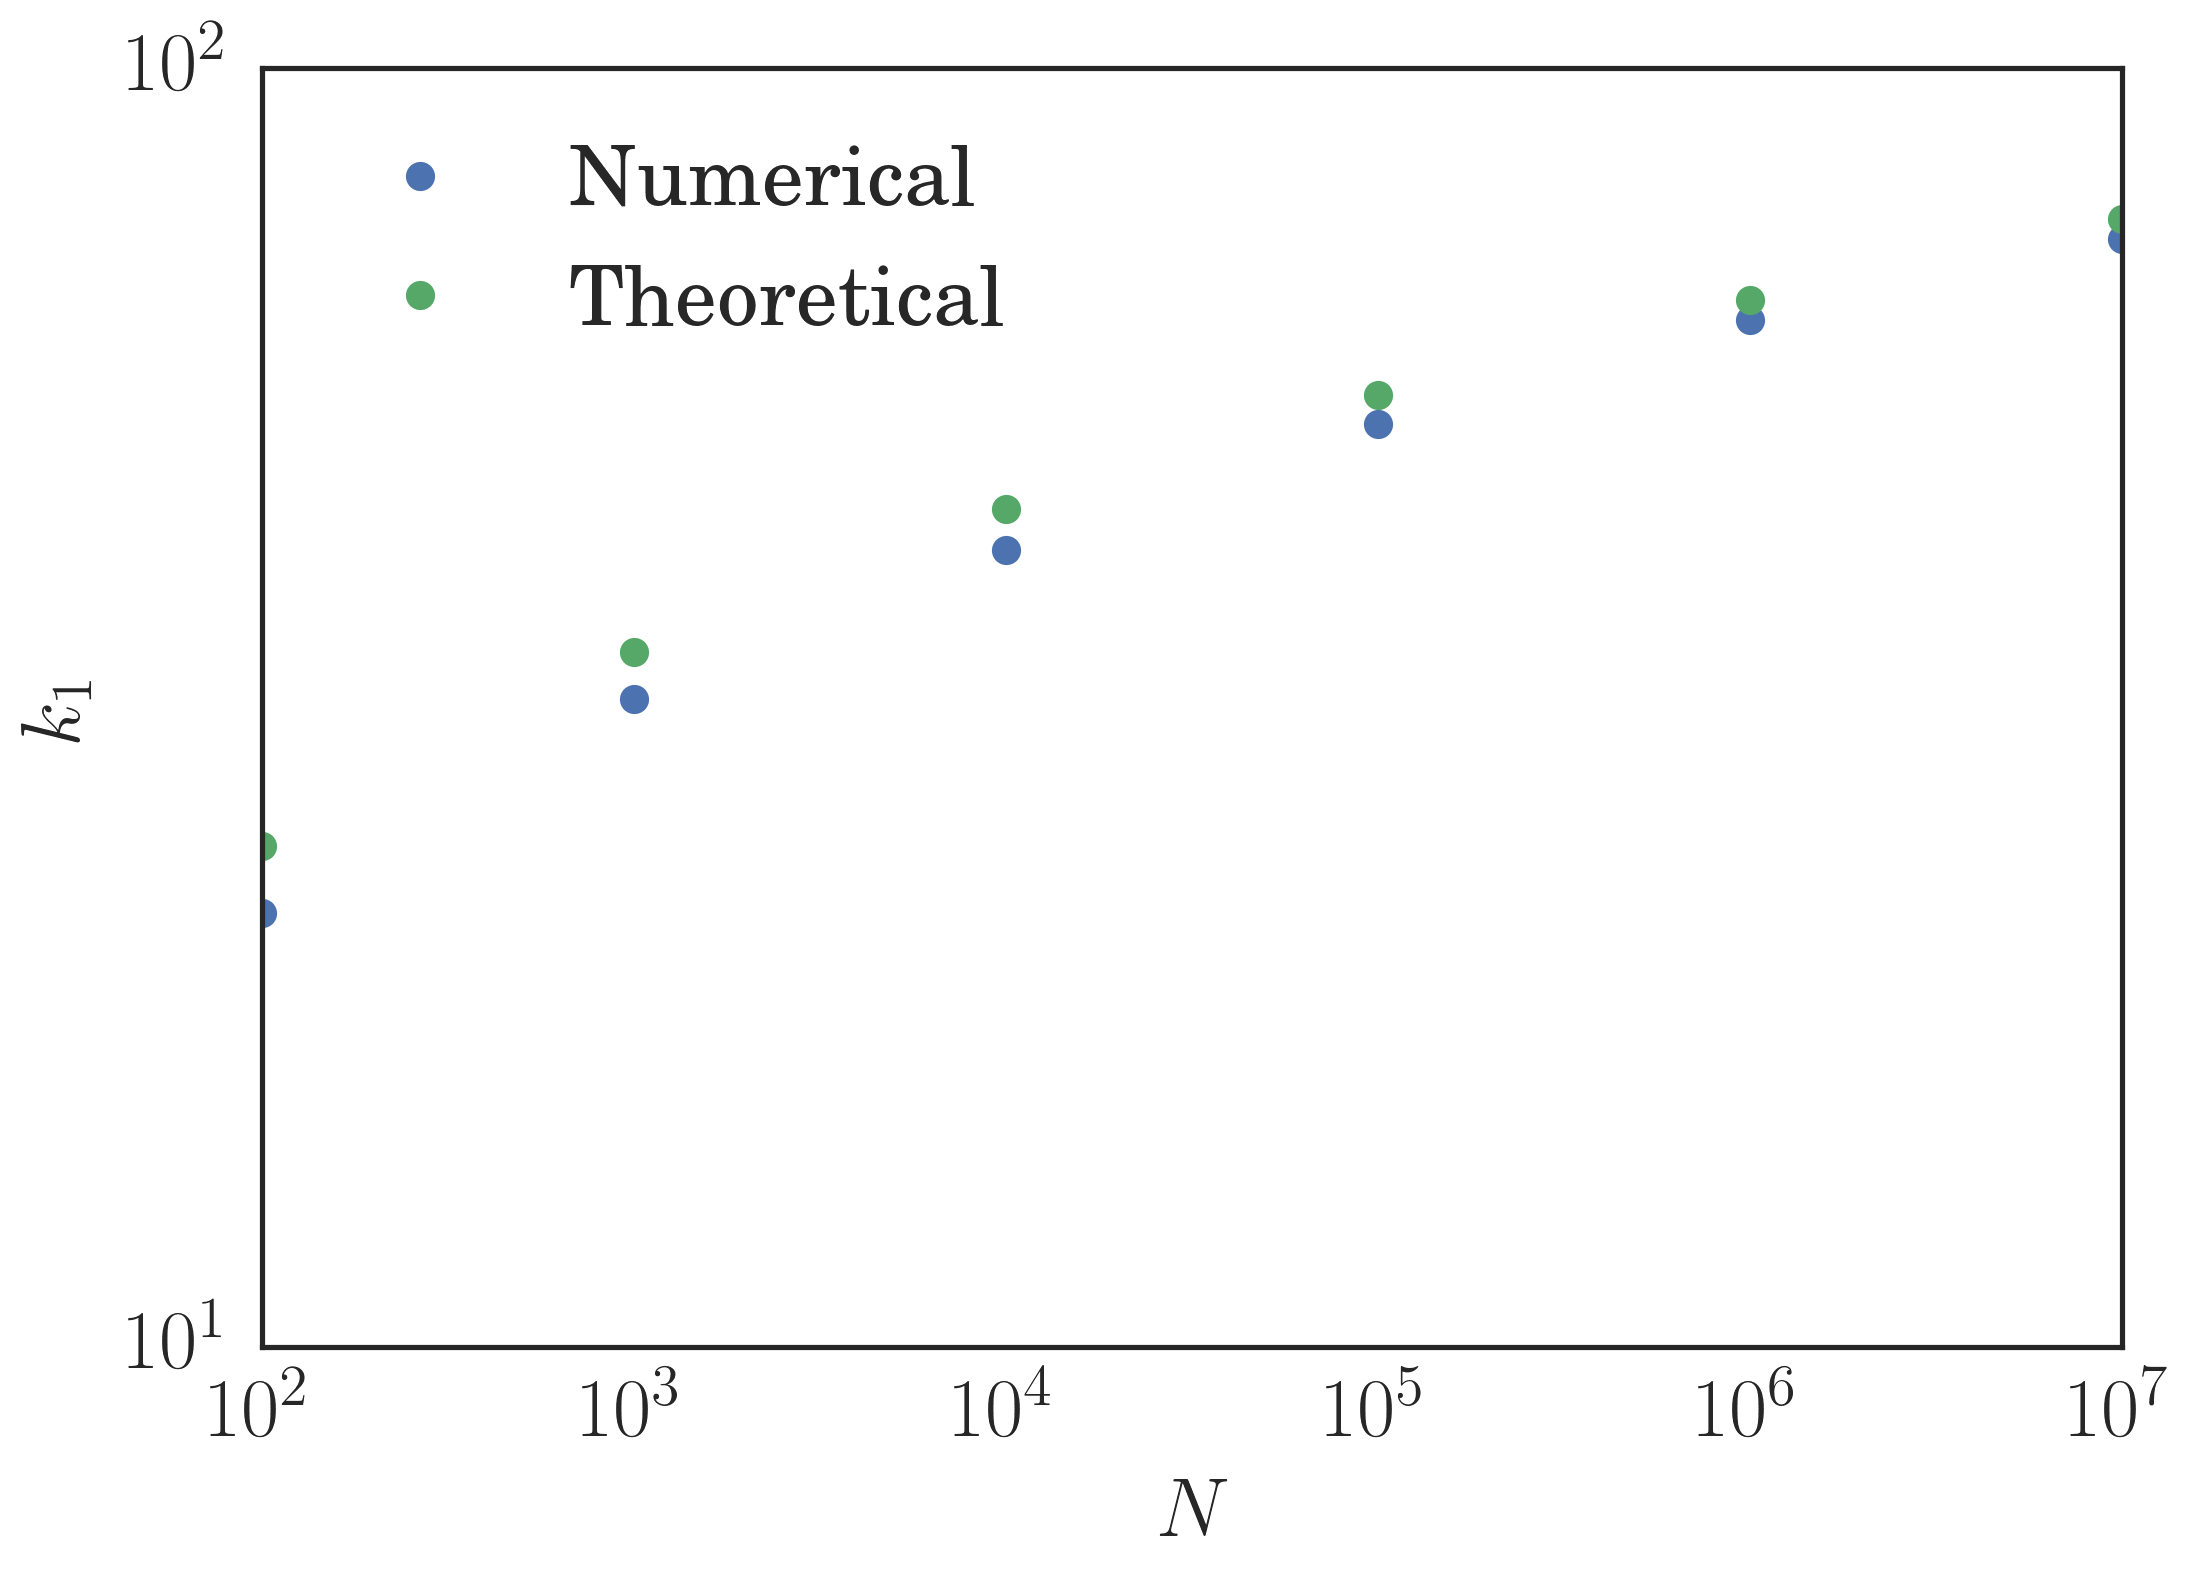
\includegraphics[height=0.5\linewidth]{img/ra-numerical-theoretical-k1}
    \caption{This shows the difference in $k_1$ for different values of $N$ ranging from $100$ to $10^7$ for random attachment. From the graph we can see that the difference between the theoretical and numerical values decrease as $N$ increases.}
    \label{fig:ra-numerical-theoretical-k1}
\end{figure}

From the following tables of values, we can also see that the values get closer to 1 for larger $N$. Similarly, the standard error was estimated from the sample standard deviation, governed by \autoref{eq:population-std}. 

\begin{center}
\begin{tabular}{ ||c | c | c | c ||}
\hline
N & $k_1^{\text{theory}}$ & $k_1^{\text{numerical}}$ & $k_1^{\text{numerical}} / k_1^{\text{theory}} $\\ 
\hline
$10^2$ & 25    & 21.85  $\pm$ 0.01 & 0.887 \\  
$10^3$ & 35   & 32.15 $\pm$ 0.03 & 0.920 \\
$10^4$ & 46   & 42.05   $\pm$  0.03  & 0.929 \\
$10^5$ & 56  & 52.75  $\pm$  0.02  & 0.949 \\
$10^6$ & 66  & 63.55  $\pm$  0.02  & 0.964 \\
$10^7$ & 76 & 73.55 $\pm$ 0.03  & 0.965 \\  
\hline
\end{tabular}
\label{table:ra-numerical-theoretical-ratio}
\captionof{table}{This table shows the theoretical and numerical values for the largest expected degree as defined in \autoref{eq:largest-degree-ra} for random attachment. The errors on $k_1$ are rounded off to 1 significant figure. }
\end{center}
%!TEX root = ../main.tex
\section{Random walks and preferential attachment}\label{section:random-walk}

\subsection{Theoretical degree distribution}
One of the weaknesses of the BA model and its generalizations is that this implicitly requires a knowledge of the total degree and a calculation across existing vertices on the graph. This requirements then destroys the potential for this model to exhibit emergent properties based on local behaviour. In real-world networks, such as social networks or webpages, the new 'vertices' that join rarely have a global knowledge of the other network vertices. The attachment by performing a random walk is a solution proposed by \citet{Saramaki2004}. In this model, a vertex is chosen at random from existing vertices and then executes a random walk of length $L$ from that vertex. The new vertex then attaches to the destination vertex. 

Preferential attachment then follows from the fact that the random walker is more likely to end up at a more highly connected vertex. This models real-world models such as interconnected webpages better, since we are likely to click on links to webpages from webpages we are already visiting. 

This model was thought to be able to reproduce the BA degree distribution even for $L=1$ \citep{Saramaki2004,J.P.Saramaki2004}. While this is the case for large $L$, \citet{Cannings2013} later showed that the $L=1$ and $m=1$ degree sequence is fundamentally different from the BA model, unless we allow an indefinite length for the random walk. 

\subsection{Numerical simulation}

A few considerations were taken into account when simulating the random walk:

\begin{enumerate}
	\item Should we reset the random walk for each new vertex added, or for each new edge we add to a vertex?
	\item Is the walk self-avoiding?
\end{enumerate}

For point 1, we followed the convention in \citet{Saramaki2004} where we continue the random walk from the previous destination vertex, until we reach $m$ destination vertices, that is, the random walk only resets when a new vertex is added. For point 2, it was decided that the walk will not be self-avoiding, otherwise it would get stuck easily. 

For $L=0$, the degree distribution reduces to that of random attachment, as expected. 

The raw degree distribution generated by $L = 1$ is shown in \autoref{fig:rw-fixed-n-degree-dist}. We can see quite clearly that the case of $m = 1$ does not follow a power law distribution of preferential attachment. 

\begin{figure}
    \centering
    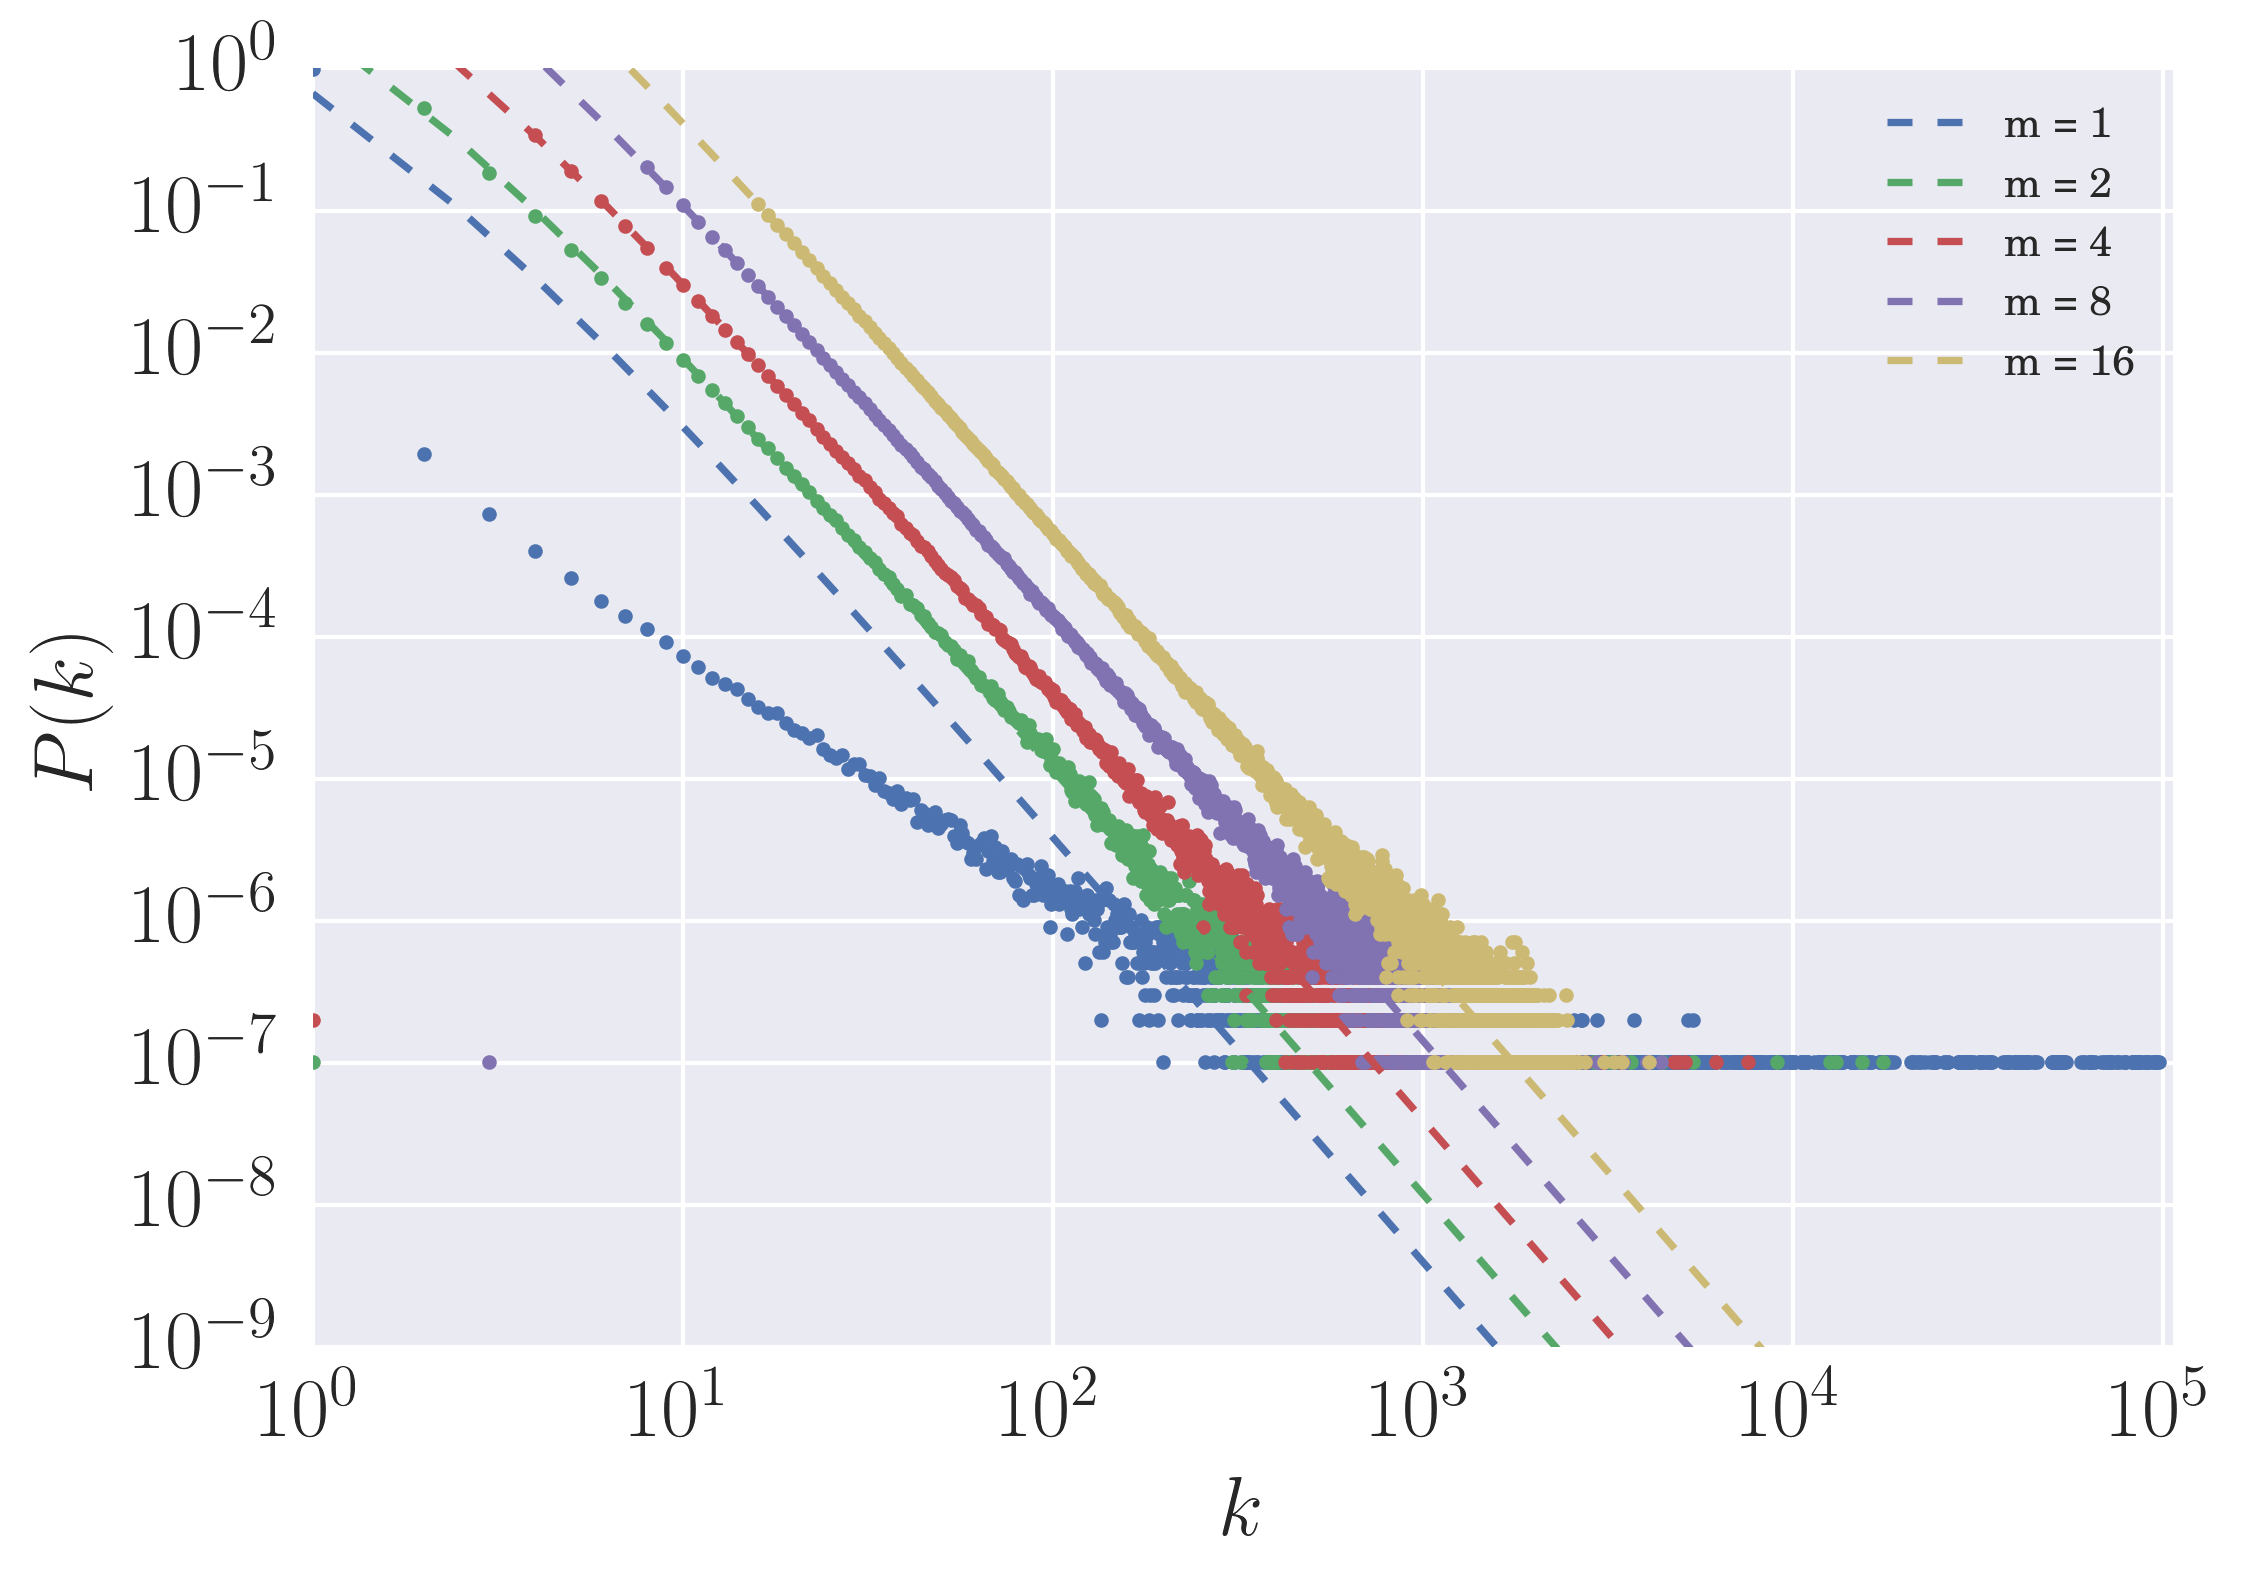
\includegraphics[height=0.5\linewidth]{img/rw-fixed-n-degree-dist}
    \caption{Degree distribution of the random walk model for $N=10^5$, $L=1$, and varying $m$. The dotted lines show the theoretical BA distribution for the same $m$. }
    \label{fig:rw-fixed-n-degree-dist}
\end{figure}

To test whether it follows a power law distribution, we can use the same technique in \autoref{subsection:ppa-numerical-analysis}. This was first done for $L=1$, $N=10^5$, and various values of $m$, and the following p-values were obtained:

\begin{center}
\begin{tabular}{ c | c}
m & $p$-value \\
\hline
1 & 0.00 \\
2 & 0.00 \\
4 & 0.029 \\
8 & 0.768 \\
16 & 0.648 \\
\end{tabular}
\label{table:rw-kstest}
\end{center} 

As we can see from the table, for small $m$. Indeed, this was verified by \citet{Cannings2013} who showed that in this case, the degree distribution converges to a degenerate limiting solution in which almost every vertex has degree 1. At $m=8$, however, it is already highly plausible that the degree distribution follows that of the preferential attachment model. 

Numerical simulations were done for fixed $N$ and $m$ but varying $L$ from 1 to 8, with the $m$ chosen to be $8$ from previous results and $N = 10^5$. The same technique was used to test whether it follows a power law distribution, and we obtain the result of $p = 0.64$ to an accuracy of $\pm 0.05$ for all $L$. This shows that it is plausible that the degree distribution for the random walk attachment follows a power law, and this holds regardless of $L$. 
The degree distributions of the BA preferential attachment model, random attachment model, and random walk model have been studied. The degree distribution for preferential attachment is a scale free power law, but this is not the case for random attachment, which is a geometric distribution. Numerical simulation results were compared with the values predicted by theory and found to be in agreement. 

\newpage
\noindent
\vspace*{2cm}

\printbibliography[heading=bibintoc]

\end{document}
